\documentclass[twocolumn]{aastex631}

\usepackage{amsmath}
\usepackage{multirow}
\usepackage{natbib}
\usepackage{graphicx} 
\usepackage{aas_macros}


\begin{document}

\title{Unveiling Cosmological Signatures in Dark Matter Halo Merger Trees: A Comparative Study of Graph Spectral Analysis, Diffusion Geometry, and Graph Neural Networks}

\author{AstroPilot}
\affiliation{Anthropic, Gemini \& OpenAI servers. Planet Earth.}

\begin{abstract}
Understanding the link between the structure of dark matter halo merger trees and the cosmological parameters that govern the Universe's evolution is a fundamental challenge. This study investigates whether graph spectral analysis and diffusion geometry can extract meaningful features from merger trees to predict the matter density parameter ($\Omega_m$) and the amplitude of matter fluctuations ($\sigma_8$). We analyzed a dataset of 1000 merger trees from N-body simulations, extracting features from the graph Laplacian spectrum, diffusion map embeddings, and astrophysically-motivated edge properties. We then trained regression models using these features and compared their performance against a baseline model using aggregated node features and a Graph Convolutional Network (GCN). While the engineered graph spectral and diffusion geometry features performed poorly, likely due to computational limitations during feature extraction, simpler aggregated node features showed significant predictive power, especially for $\Omega_m$. The GCN model achieved the best performance, demonstrating the potential of graph neural networks to automatically learn cosmologically relevant information directly from merger tree structures, highlighting the challenges of manual feature engineering in complex graph data and the promise of geometric deep learning for cosmological inference.
\
\end{abstract}

\keywords{N-body simulations, Dimensionality reduction, Dark matter, Regression, Cosmological parameters}


\section{Introduction}
\label{sec:intro}
Understanding the formation and evolution of cosmic structures is a cornerstone of modern cosmology. Dark matter halos, the scaffolding upon which galaxies form, grow through a hierarchical process of mergers and accretion, leaving a trace of their history in the form of merger trees. These trees, representing the ancestral lineage of a halo, are thought to encode valuable information about the underlying cosmological parameters that govern the Universe's evolution, such as the matter density parameter ($\Omega_m$) and the amplitude of matter fluctuations ($\sigma_8$). Therefore, extracting cosmological information from the complex architecture of merger trees is a key challenge in modern cosmology.

However, the inherent complexity and variability of merger trees pose significant analytical hurdles. Merger trees are naturally represented as graphs, with nodes representing halos and edges representing merger events \citep{parkinson2007generatingdarkmatterhalo,robles2022deeplearningapproachhalo}. These graphs vary substantially in size and structure, making it difficult to apply traditional machine learning techniques that require fixed-size feature vectors \citep{robles2022deeplearningapproachhalo}. Furthermore, the relationships between merger tree morphology and cosmological parameters are likely complex and non-linear, making it difficult to identify the most informative features for cosmological inference \citep{geda2025constructingmergertreesdensity}. Traditional approaches often rely on hand-engineered features that summarize global properties of the trees, potentially missing subtle but important relationships between the merger history and cosmological parameters \citep{parkinson2007generatingdarkmatterhalo,jung2024mergertreebasedgalaxymatching}.

In this work, we explore the application of graph signal processing techniques, specifically graph spectral analysis and diffusion geometry, to extract cosmologically relevant information from dark matter halo merger trees. Our approach is based on the hypothesis that the spectral properties of the graph Laplacian and the diffusion geometry of merger trees encode robust, interpretable, and computationally efficient features that can be used to predict cosmological parameters. The graph Laplacian provides a way to characterize the connectivity and structure of a graph through its eigenvalues and eigenvectors. Diffusion geometry, on the other hand, provides a way to embed the nodes of a graph into a low-dimensional space that captures the diffusion dynamics on the graph. We hypothesize that the eigenvalues and eigenvectors of the graph Laplacian, as well as the low-dimensional embeddings obtained through diffusion maps, capture the overall connectivity and structural properties of the merger trees in a way that is sensitive to the underlying cosmology.

To test this hypothesis, we analyze a dataset of 1000 merger trees extracted from N-body simulations \citep{bose2022constructinghighfidelityhalomerger}. We extract features from the graph Laplacian spectrum, diffusion map embeddings, and astrophysically-motivated edge properties, such as the scale factor difference and mass ratio between merging halos \citep{bose2022constructinghighfidelityhalomerger,chandrogómez2025accuracydarkmatterhalo}. We then train regression models using these features to predict $\Omega_m$ and $\sigma_8$ \citep{chandrogómez2025accuracydarkmatterhalo}. We compare the performance of these models against two baselines: a model using simpler, aggregated node features and a Graph Convolutional Network (GCN) \citep{bose2022constructinghighfidelityhalomerger,jung2024mergertreebasedgalaxymatching}. The first baseline serves to test whether sophisticated graph features outperform simple global statistics of node properties \citep{bose2022constructinghighfidelityhalomerger}. The GCN serves as a benchmark for assessing the potential of geometric deep learning to automatically learn cosmologically relevant features directly from the merger tree structures, bypassing the need for manual feature engineering. By comparing the performance of these different approaches, we aim to evaluate the effectiveness of graph spectral analysis and diffusion geometry for extracting cosmologically relevant information from dark matter halo merger trees and to compare the performance of these methods to simpler feature engineering approaches and more sophisticated graph neural networks \citep{bose2022constructinghighfidelityhalomerger,jung2024mergertreebasedgalaxymatching,chandrogómez2025accuracydarkmatterhalo}.
\
\

\section{Methods}
\label{sec:methods}
\subsection{Data Acquisition and Preprocessing}
\subsubsection{Dataset Description}
The foundation of our analysis rests on a dataset comprising 1000 dark matter halo merger trees. These trees were extracted from N-body simulations, capturing the hierarchical formation history of dark matter halos. Each merger tree is structured as a directed acyclic graph, where nodes represent dark matter halos at different points in time, and edges signify merger events between halos. The dataset is conveniently stored in the PyTorch Geometric format, a library designed for handling graph-structured data. Each `Data` object within the dataset encapsulates the following crucial information:
\begin{itemize}
    \item \textbf{Node Features (`x`)}: A matrix of shape `[num\_nodes, 4]` containing four key properties for each halo (node): the base-10 logarithm of the halo mass (log10(mass)), the base-10 logarithm of the halo concentration (log10(concentration)), the base-10 logarithm of the maximum circular velocity (log10(Vmax)), and the cosmological scale factor at the time the halo existed.
    \item \textbf{Edge Index (`edge\_index`)}: A matrix of shape `[2, num\_edges]` that defines the graph's connectivity, specifying the source and target nodes for each merger event (edge).
    \item \textbf{Edge Attributes (`edge\_attr`)}: A matrix of shape `[num\_edges, 1]` that stores a single feature associated with each merger event. This feature's precise nature will be carefully examined during exploratory data analysis (EDA), and if it proves insufficient for our purposes, we will compute astrophysically motivated edge features from the node properties.
    \item \textbf{Graph-Level Labels (`y`)}: A matrix of shape `[1, 2]` containing the cosmological parameters associated with the simulation from which the merger tree was extracted: the matter density parameter ($\Omega_m$) and the amplitude of matter fluctuations ($\sigma_8$). These are the target variables for our regression models.
    \item \textbf{Number of Nodes (`num\_nodes`)}: The total number of halos (nodes) in the merger tree.
    \item \textbf{Latin Hypercube ID (`lh\_id`)}: An identifier indicating the specific Latin Hypercube simulation from which the merger tree originated. This is crucial for ensuring simulation-aware data splitting.
    \item \textbf{Node Halo ID (`node\_halo\_id`)}: Unique identifiers for each halo (node) within the merger tree.
\end{itemize}

\subsubsection{Exploratory Data Analysis}
Prior to feature engineering and model training, we conducted a comprehensive exploratory data analysis (EDA) to gain a thorough understanding of the dataset's characteristics.
This involved examining the distributions of node features, target variables, and graph structural properties \citep{haghighi2023analyzingastronomicaldatamachine}.
The EDA process included:
\begin{enumerate}
    \item \textbf{Node Feature Distributions}: Analyzing the distributions of the four node features (log10(mass), log10(concentration), log10(Vmax), scale factor) across all nodes in all 1000 merger trees. This step is critical for identifying potential outliers, understanding the ranges of feature values, and informing subsequent normalization procedures.
    \item \textbf{Graph Target Variable Distributions}: Examining the distributions of the cosmological parameters ($\Omega_m$ and $\sigma_8$). Given that the dataset comprises 1000 merger trees originating from 40 unique simulations (with 25 trees per simulation), the target variables (`y`) remain constant for all trees derived from the same simulation (`lh\_id`). This analysis helps confirm the expected ranges and variability of the target variables.
    \item \textbf{Graph Structural Properties}: Analyzing the distribution of graph sizes, specifically the number of nodes and edges in each merger tree. This is important because the variability in graph size necessitates the use of graph embedding methods that can produce fixed-size representations.
    \item \textbf{Edge Attribute Investigation}: Examining the nature and distribution of the provided `edge\_attr`. If this attribute is not directly interpretable as a physical quantity relevant to merger events, we will proceed to compute these features manually as described later.
\end{enumerate}
\citep{kent2017editorialtechniquesmethodsastrophysical,giri2025astronomycalcpythontoolkitteaching}

\subsubsection{Data Splitting}
To ensure robust and unbiased model evaluation, the dataset was split into training and testing sets \citep{frailis2004perspectsastrophysicaldatabases,onose2016scalablesplittingalgorithmsbigdata}. Critically, this split was performed at the simulation level using the `lh\_id` to prevent data leakage, as all trees from the same simulation share identical $\Omega_m$ and $\sigma_8$ values. A `GroupShuffleSplit` from scikit-learn was employed to achieve this, ensuring that all trees from a given simulation were assigned to either the training or testing set. We used an 80/20 split, where 80\% of the unique simulations were used for training and the remaining 20\% for testing.

\subsubsection{Feature Normalization}
To improve model performance and stability, node features (`x`) were normalized using `StandardScaler` from scikit-learn \citep{bhowmik2024imageprocessinganalysismultiple}. The mean and standard deviation for each of the four node features were calculated *solely from the training set graphs*. This ensures that the testing set is normalized using statistics derived from the training data, preventing data leakage \citep{różański2021suppnetneuralnetworkstellar}. The normalization transformation was then applied to both the training and testing sets. Target variables `y` ($\Omega_m$, $\sigma_8$) were not normalized, as tree-based regressors like Random Forest and Gradient Boosting are generally insensitive to the scale of the target variable \citep{stonemartinez2025starflowleveragingnormalizingflows}.

\subsection{Feature Engineering from Merger Trees}
For each graph in the dataset, we extracted three distinct sets of features: graph spectral features \citep{jespersen2022textttmangrovelearninggalaxyproperties,bose2022constructinghighfidelityhalomerger}, diffusion geometry embeddings \citep{robles2022deeplearningapproachhalo}, and astrophysically-motivated edge feature aggregations \citep{gómez2021halomergertreecomparison}. Each of these sets aims to capture different aspects of the merger tree structure and the underlying physical processes.

\subsubsection{Graph Spectral Feature Extraction}
Graph spectral features capture the global connectivity and structure of the merger trees by analyzing the eigenvalues of the graph Laplacian \citep{desouza2023graphbasedspectralclassificationtype,pavlou2023graphtheoreticalanalysislocal}.
\begin{enumerate}
    \item \textbf{Normalized Graph Laplacian Computation}: For each graph $g = (V, E)$, we first converted the `edge\_index` to a SciPy sparse adjacency matrix $A$. We then computed the normalized graph Laplacian, defined as $L_{norm} = I - D^{-1/2} A D^{-1/2}$, where $D$ is the diagonal degree matrix and $I$ is the identity matrix. The normalization ensures that the eigenvalues of $L_{norm}$ lie in the interval $[0, 2]$, providing a stable basis for spectral analysis.
    \item \textbf{Eigenvalue Decomposition}: We computed the eigenvalues of $L_{norm}$ using the `scipy.sparse.linalg.eigsh` function, which is optimized for sparse matrices. Given the varying sizes of the graphs, storing all eigenvalues for each graph would result in variable-length feature vectors.
    \item \textbf{Spectral Moment Calculation}: To obtain a fixed-size feature vector for each graph, we computed spectral moments from its eigenvalue distribution. Specifically, we calculated the first four central moments: the mean, standard deviation, skewness, and kurtosis of the eigenvalues. Additionally, we calculated the sum of the smallest $m=10$ non-zero eigenvalues (if available, padded with zeros if fewer than 10 non-zero eigenvalues existed). These spectral moments provide a compact summary of the shape of the eigenvalue distribution, capturing key structural properties of the graph.
\end{enumerate}

\subsubsection{Diffusion Geometry Embedding}
Diffusion geometry provides an alternative approach to characterizing graph structure by embedding nodes in a low-dimensional space that reflects the diffusion dynamics on the graph \citep{berger2017visualizingtimevaryingparticleflows,jagvaral2023unifiedframeworkdiffusiongenerative}.
\begin{enumerate}
    \item \textbf{Diffusion Operator Construction}: For each graph, we constructed a diffusion operator using the random walk transition matrix $P = D^{-1}A$, where $D$ is the diagonal degree matrix and $A$ is the adjacency matrix. This matrix represents the probability of transitioning between connected nodes in one step of a random walk.
    \item \textbf{Eigenvector Computation for Node Embeddings}: We computed the eigenvectors of $P$ and selected the top $d$ eigenvectors corresponding to the largest eigenvalues (excluding the trivial eigenvector for eigenvalue 1, if present). We experimented with $d=3$ and $d=5$ to assess the sensitivity of the results to the embedding dimensionality. These eigenvectors form a $d$-dimensional embedding for each node in the graph, capturing its position within the graph's diffusion geometry.
    \item \textbf{Graph-Level Aggregation of Node Embeddings}: To obtain a fixed-size feature vector for each graph, we aggregated the $d$-dimensional node embeddings using mean pooling, max pooling, and min pooling. These operations compute the element-wise mean, maximum, and minimum of the node embeddings, respectively. The resulting vectors were then concatenated to form a single graph-level feature vector of length $3d$. For example, with $d=3$, the resulting feature vector would have a length of 9. This aggregation summarizes the distribution of node positions in the diffusion embedding space, providing a global representation of the graph's structure.
\end{enumerate}

\subsubsection{Astrophysically-Motivated Edge Feature Aggregation}
These features aim to capture relevant aspects of the merger events within the merger trees, focusing on the physical properties of the merging halos \citep{jespersen2022textttmangrovelearninggalaxyproperties,jung2024mergertreebasedgalaxymatching,chandrogómez2025accuracydarkmatterhalo}.
\begin{enumerate}
    \item \textbf{Calculation of Edge-Level Physical Properties}: For each edge $(u, v)$ in a merger tree, representing a progenitor halo $u$ merging into a descendant halo $v$, we calculated the following properties:
    \begin{itemize}
        \item \textbf{Scale Factor Difference}: $\Delta_{sf} = |scale\_factor(u) - scale\_factor(v)|$. Since edges point from progenitors to descendants, we expect $scale\_factor(v) > scale\_factor(u)$, and $\Delta_{sf}$ represents the time interval between the merger event and the observation time.
        \item \textbf{Log Mass Ratio}: $log\_mass\_ratio = log10(mass(v)) - log10(mass(u))$, representing the ratio of the descendant halo mass to the progenitor halo mass. This quantity reflects the mass accretion during the merger event.
    \end{itemize}
    \item \textbf{Aggregation to Graph-Level Statistics}: For each graph, we calculated the mean and variance of $\Delta_{sf}$ and $log\_mass\_ratio$ over all its edges. This resulted in four features per graph: the mean and variance of the scale factor difference, and the mean and variance of the log mass ratio. These statistics provide a summary of the typical and atypical merger event characteristics within a tree.
\end{enumerate}

\subsection{Model Development and Evaluation}
\subsubsection{Feature Vector Assembly and Dimensionality Reduction}
For each graph, we concatenated the features derived from graph spectral moments, aggregated diffusion map embeddings, and aggregated astrophysically-motivated edge statistics \citep{sun2024knowledgegraphastronomicalresearch}. This resulted in a single, high-dimensional feature vector per merger tree. To reduce dimensionality, decorrelate features, and potentially improve model performance, we applied Principal Component Analysis (PCA) to the combined feature vectors derived from the training set \citep{ma2025characterizingdarkmattersubhalo}. The number of principal components to retain was determined by the amount of variance explained (e.g., 95\% or 99\%). Both training and testing set feature vectors were then transformed using the fitted PCA.

\subsubsection{Regression Models for Cosmological Parameter Prediction}
We trained separate regression models to predict $\Omega_m$ and $\sigma_8$ \citep{villaescusanavarro2021camelsprojectcosmologyastrophysics}. We explored two different regression models: Random Forest Regressor and Gradient Boosting Regressor (specifically, XGBoost and LightGBM). These models were chosen for their robustness, ability to capture non-linear relationships, and relatively low computational cost \citep{villaescusanavarro2021camelsprojectcosmologyastrophysics,balla2024cosmicscalebenchmarksymmetrypreservingdata,makinen2024hybridsummarystatistics}.

\subsubsection{Training and Hyperparameter Optimization}
The selected models were trained on the PCA-transformed feature vectors from the training set \citep{steiner2009pcatomographyextractinformation,yun2023pcafilteringmethodunbiased,kuiper2025representationlearningfastradio}. Hyperparameter optimization was performed using cross-validation on the training set. To ensure that the cross-validation process did not introduce data leakage, the cross-validation splits were also performed at the simulation level, respecting the `lh\_id` groupings. We employed `GridSearchCV` or `RandomizedSearchCV` to search for the optimal hyperparameter settings for each model.

\subsubsection{Evaluation Metrics}
The performance of the trained models was evaluated on the test set using the following metrics: \citep{mishrasharma2024paperclipassociatingastronomicalobservations,narkedimilli2024predictingstellarmetallicitycomparative,raghav2024photometricanalysispredictingstar}.
\begin{itemize}
    \item \textbf{R-squared (R²)}: The coefficient of determination, which measures the proportion of variance in the target variable that is explained by the model.
    \item \textbf{Mean Squared Error (MSE)}: The average squared difference between the predicted and actual values.
\end{itemize}
If the models provided uncertainty estimates (e.g., quantile regression for Gradient Boosting, or variance from Random Forests), we assessed their calibration using Expected Calibration Error (ECE) \citep{pandya2025siddasinkhorndynamicdomain} and reliability diagrams. These metrics evaluate the consistency between the predicted probabilities/quantiles and the observed frequencies.

\subsubsection{Baseline Models for Comparison}
To provide context for the performance of our proposed feature set, we compared our results against two baseline models \citep{pan2024astromlab2astrollama270bmodel,dehaan2025astromlab3achievinggpt4o}.
\begin{enumerate}
    \item \textbf{Baseline 1: Aggregated Node Features with Classical Regressors}
For each graph, we computed simple aggregated node features: mean, standard deviation, minimum, and maximum for each of the four raw node features (log10(mass), log10(concentration), log10(Vmax), scale factor). This resulted in a 16-dimensional feature vector per graph. We then trained Random Forest and Gradient Boosting regressors on these aggregated features, using the same training/testing split and hyperparameter optimization strategy as before \citep{soo2023machinelearningapplicationsastrophysics}. This baseline tests whether sophisticated graph features outperform simple global statistics of node properties.
    \item \textbf{Baseline 2: Graph Convolutional Network (GCN)}
We implemented a simple Graph Convolutional Network (GCN) for graph-level regression. The GCN architecture consisted of 2-3 `GCNConv` layers with ReLU activations, followed by a global mean pooling layer to obtain a graph-level embedding, and an MLP (2 fully connected layers) to regress $\Omega_m$ and $\sigma_8$ \citep{zhong2024improvingconvolutionalneuralnetworks,kvasiuk2024reconstructioncontinuouscosmologicalfields}. The GCN was trained on the training graph data using the MSE loss function. The training process was performed on CPUs. This baseline compares our "classical" graph feature engineering approach against a common geometric deep learning model.
\end{enumerate}

\section{Results}
\label{sec:results}
\subsection{Data Preprocessing and Feature Engineering}

The initial dataset consisted of 1000 merger trees, originating from 40 unique N-body simulations, with 25 trees per simulation. Prior to feature engineering, node features, specifically the base-10 logarithm of halo mass (log10(mass)), the base-10 logarithm of halo concentration (log10(concentration)), the base-10 logarithm of the maximum circular velocity (log10(Vmax)), and the cosmological scale factor, were normalized. This normalization was performed using the mean and standard deviation computed solely from the training set (800 trees from 32 simulations). The computed normalization parameters, detailed in the file `data/normalization\_params.npz`, were: mean = `[11.138, 0.736, 2.115, 0.370]` and std = `[0.713, 0.364, 0.212, 0.180]` for the four node features, respectively.

A total of 24 engineered features were constructed for each graph, divided into three categories:
\begin{enumerate}
    \item Edge-based features (4): These features captured information about the merger events. They included the mean and variance of the absolute difference in scale factors between connected nodes, and the mean and variance of the log-ratio of descendant mass to progenitor mass.
    \item Laplacian spectral features (5): These features aimed to capture the global connectivity and structure of the merger trees. They included the mean, standard deviation, skewness, and kurtosis of the normalized graph Laplacian eigenvalues, as well as the sum of the 10 smallest non-zero eigenvalues.
    \item Diffusion map features (15): These features were derived from node embeddings obtained using diffusion maps. The top 5 eigenvectors of the random walk transition matrix were used to embed the nodes, and these embeddings were then aggregated at the graph level using mean, maximum, and minimum pooling (5 eigenvectors x 3 aggregation methods).
\end{enumerate}

A significant challenge was the computational cost associated with eigenvalue decomposition for large graphs. To address this, a threshold (`MAX\_NODES\_FOR\_EIGS = 500`) was set, above which Laplacian and diffusion feature calculations were skipped. This resulted in NaN values for these features in graphs exceeding this size limit. Specifically, 638 out of 800 training graphs and 164 out of 200 test graphs exceeded this limit. Consequently, a substantial number of NaN entries were present in the engineered feature matrices (12,760 NaNs in `X\_train\_engineered` (an 800x24 matrix) and 3,280 NaNs in `X\_test\_engineered` (a 200x24 matrix)), primarily affecting the 20 spectral and diffusion features. These NaNs were subsequently handled by mean imputation prior to Principal Component Analysis (PCA).

The distributions of the engineered features (post-imputation for plotting purposes where applicable, using raw values from `data/engineered\_features\_train.npz`) were visualized in a series of histograms. The distributions of the edge features, such as `mean\_\_delta\_\_sf` and `mean\_\_log\_\_mass\_\_ratio`, are shown in Figure \ref{fig:edge_feature_dist} and were relatively compact. However, the distributions of the Laplacian spectral features (e.g., `lap\_\_eig\_\_mean` and `lap\_\_eig\_\_std`) and the diffusion map features (mean, max, min pooled) were significantly influenced by the imputation of NaNs for large graphs, as illustrated in Figures \ref{fig:laplacian_feature_dist}, \ref{fig:diffusion_feature_dist_mean}, \ref{fig:diffusion_feature_dist}, and \ref{fig:diffusion_feature_dist_min}.

\begin{figure}[h!]
    \centering
    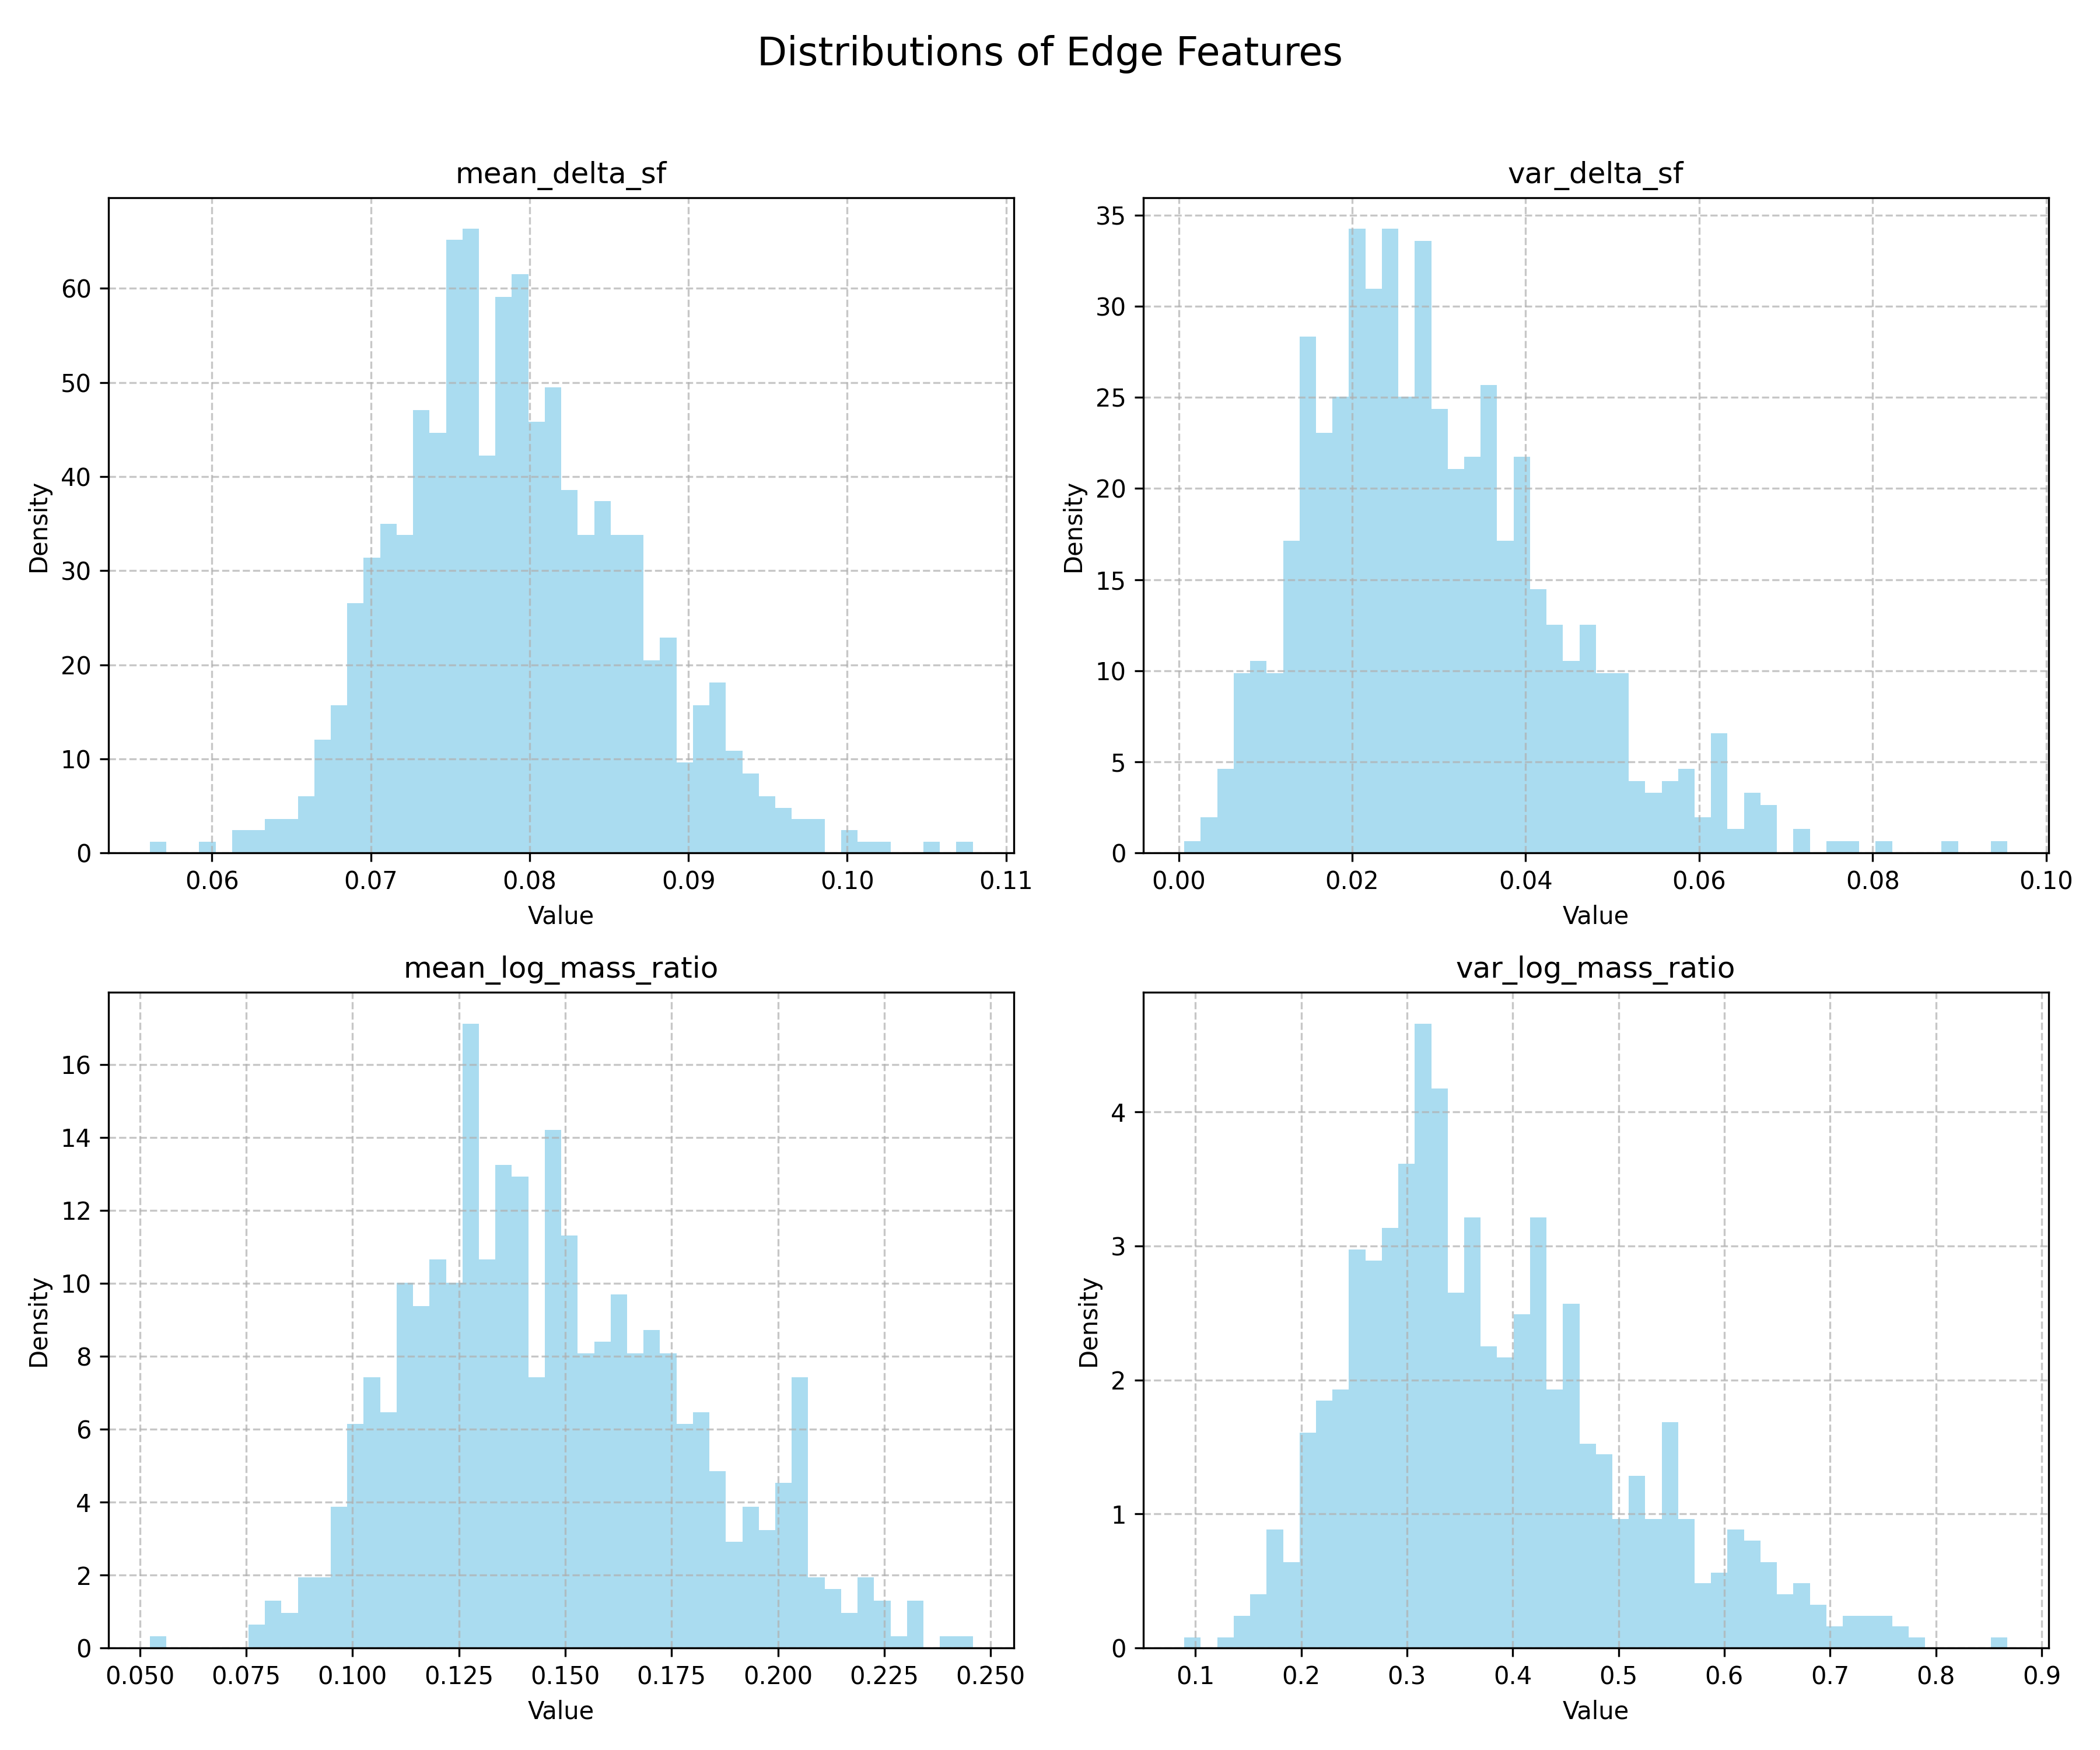
\includegraphics[width=0.5\textwidth]{../input_files/plots/engineered_feature_dist_edge_1_20250527-135752.png}
    \caption{Distributions of edge features (mean and variance of the absolute difference in scale factors between connected nodes, and mean and variance of the log-ratio of descendant mass to progenitor mass). These relatively compact distributions were used to predict cosmological parameters, but ultimately performed worse than simpler features.}
    \label{fig:edge_feature_dist}
\end{figure}

\begin{figure}[h!]
    \centering
    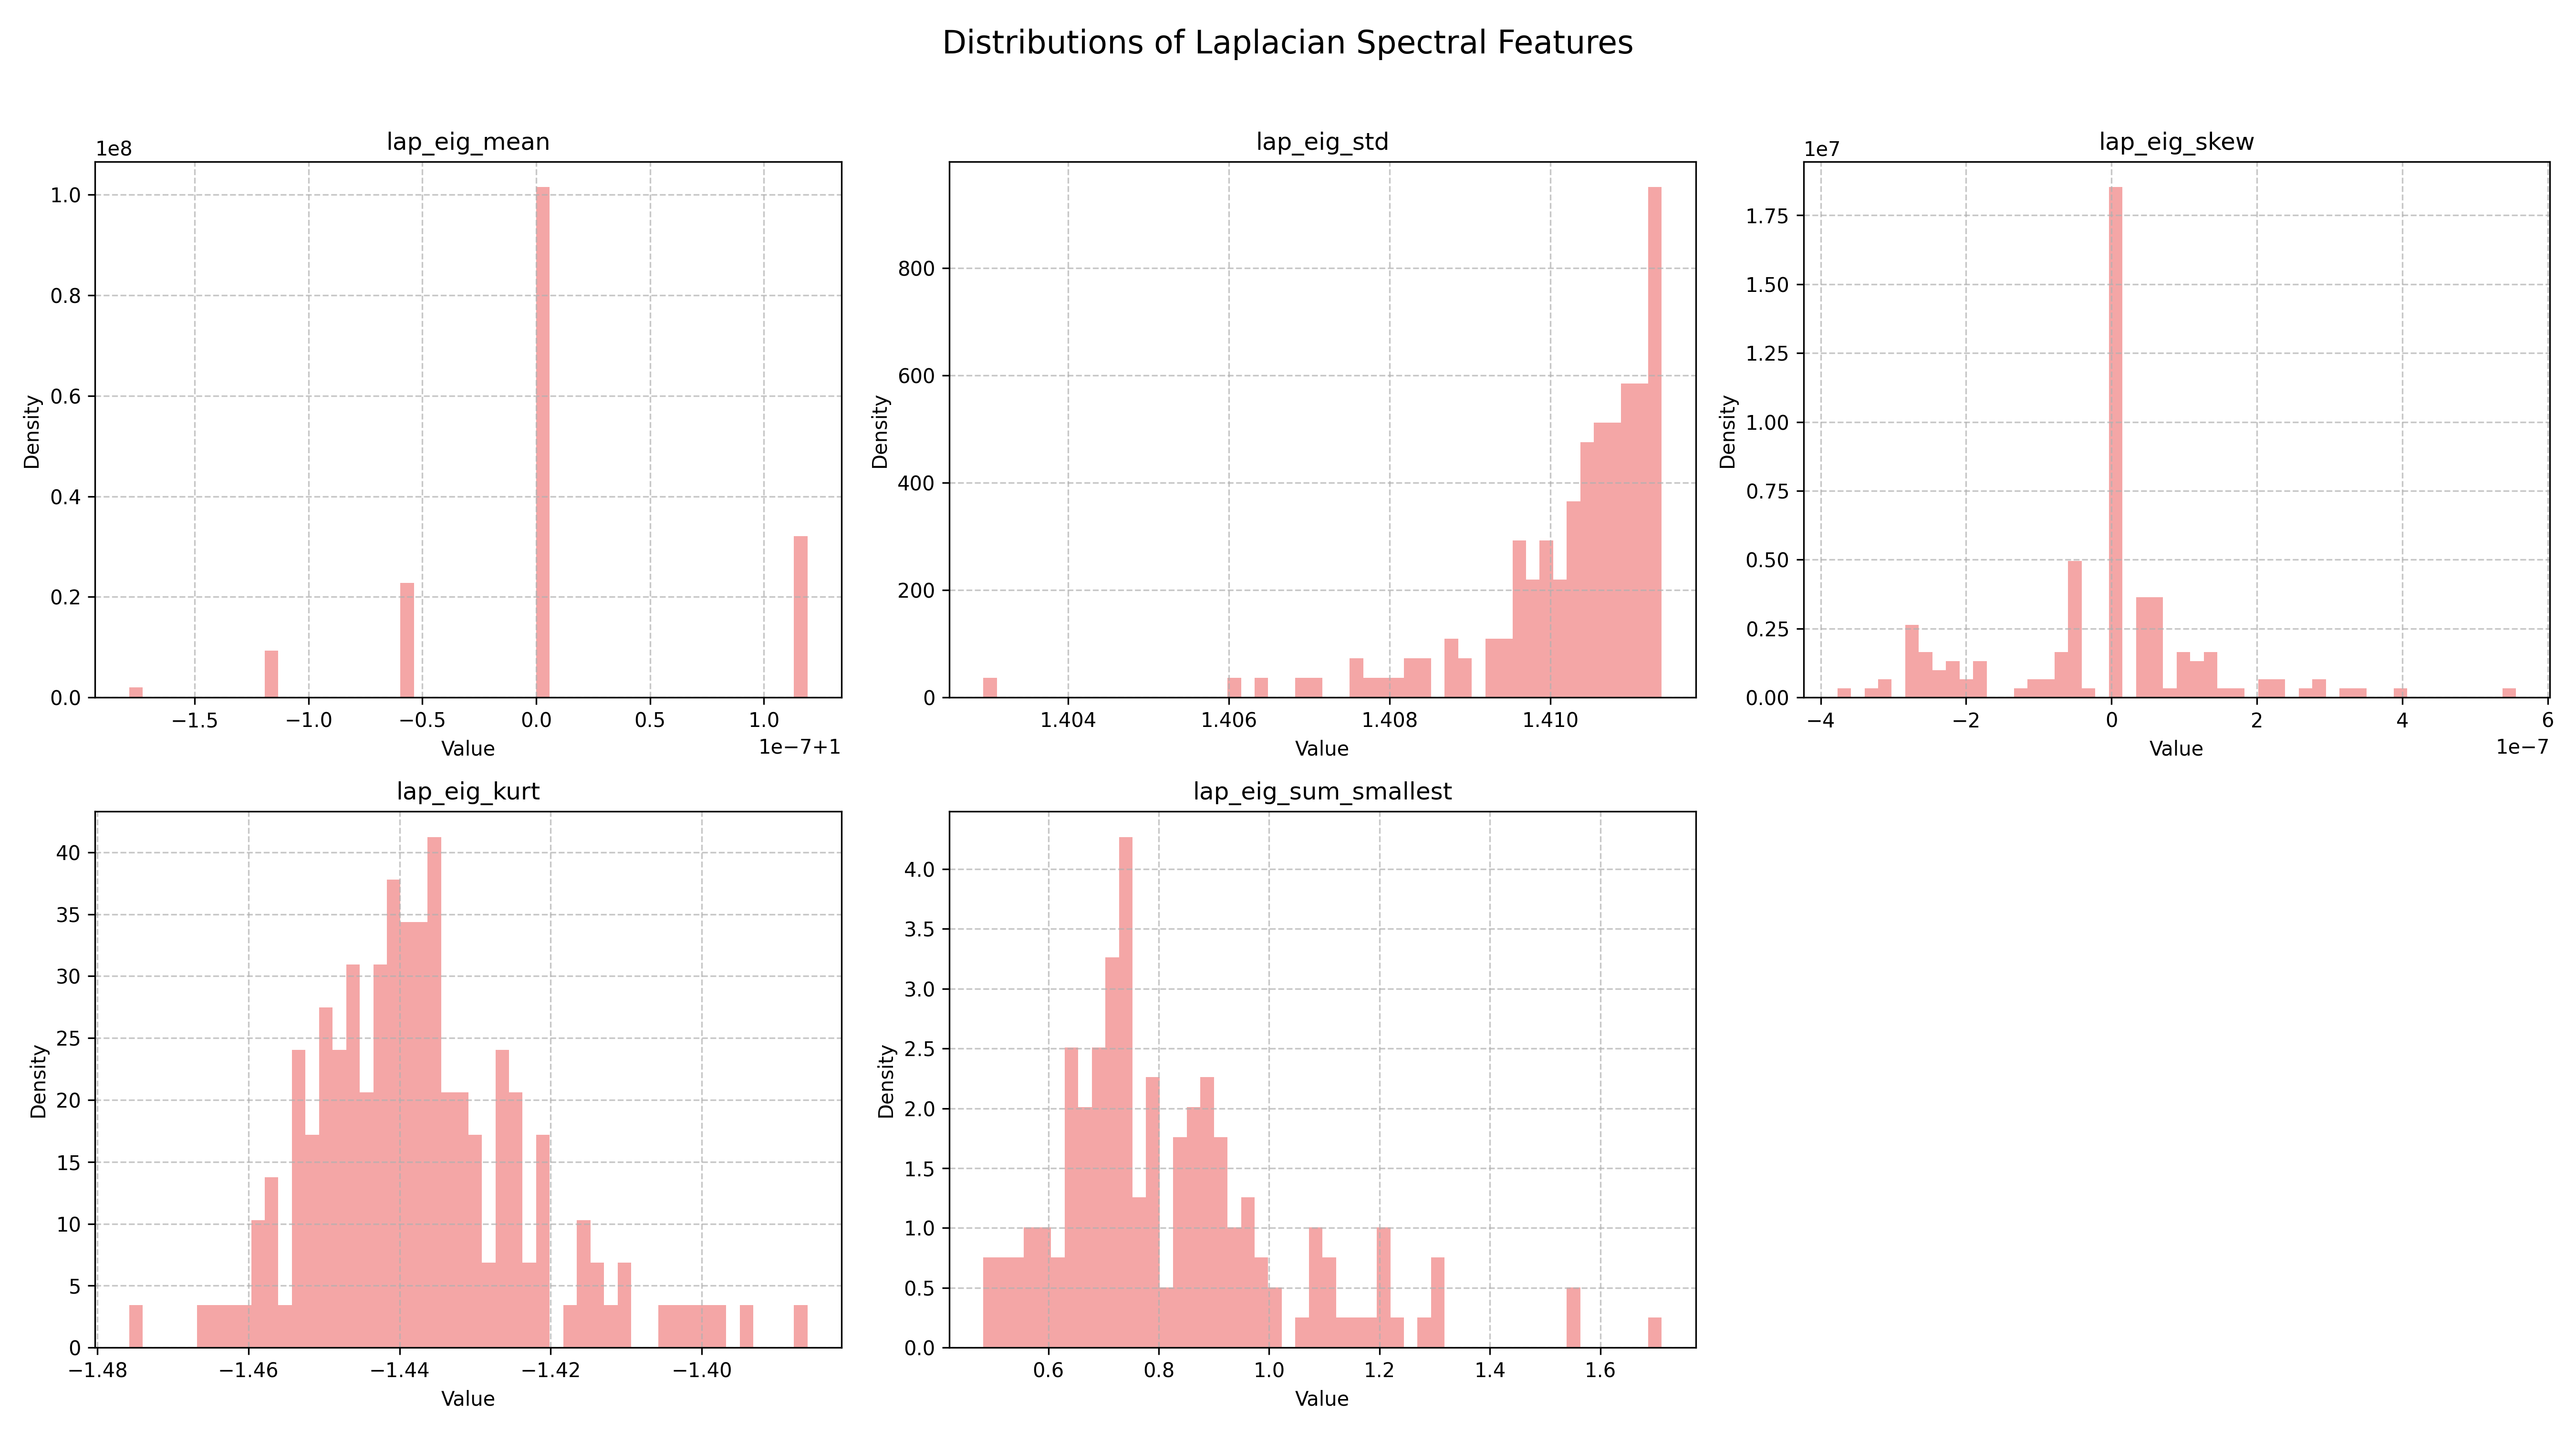
\includegraphics[width=0.5\textwidth]{../input_files/plots/engineered_feature_dist_laplacian_2_20250527-135752.png}
    \caption{Distributions of Laplacian spectral features (mean, standard deviation, skewness, kurtosis, and sum of the 10 smallest non-zero eigenvalues) across the training set merger trees. These features, intended to capture graph structure, were ultimately found to be poor predictors of cosmological parameters, likely due to the imputation of NaN values arising from computational limitations for large graphs.}
    \label{fig:laplacian_feature_dist}
\end{figure}

\begin{figure}[h!]
    \centering
    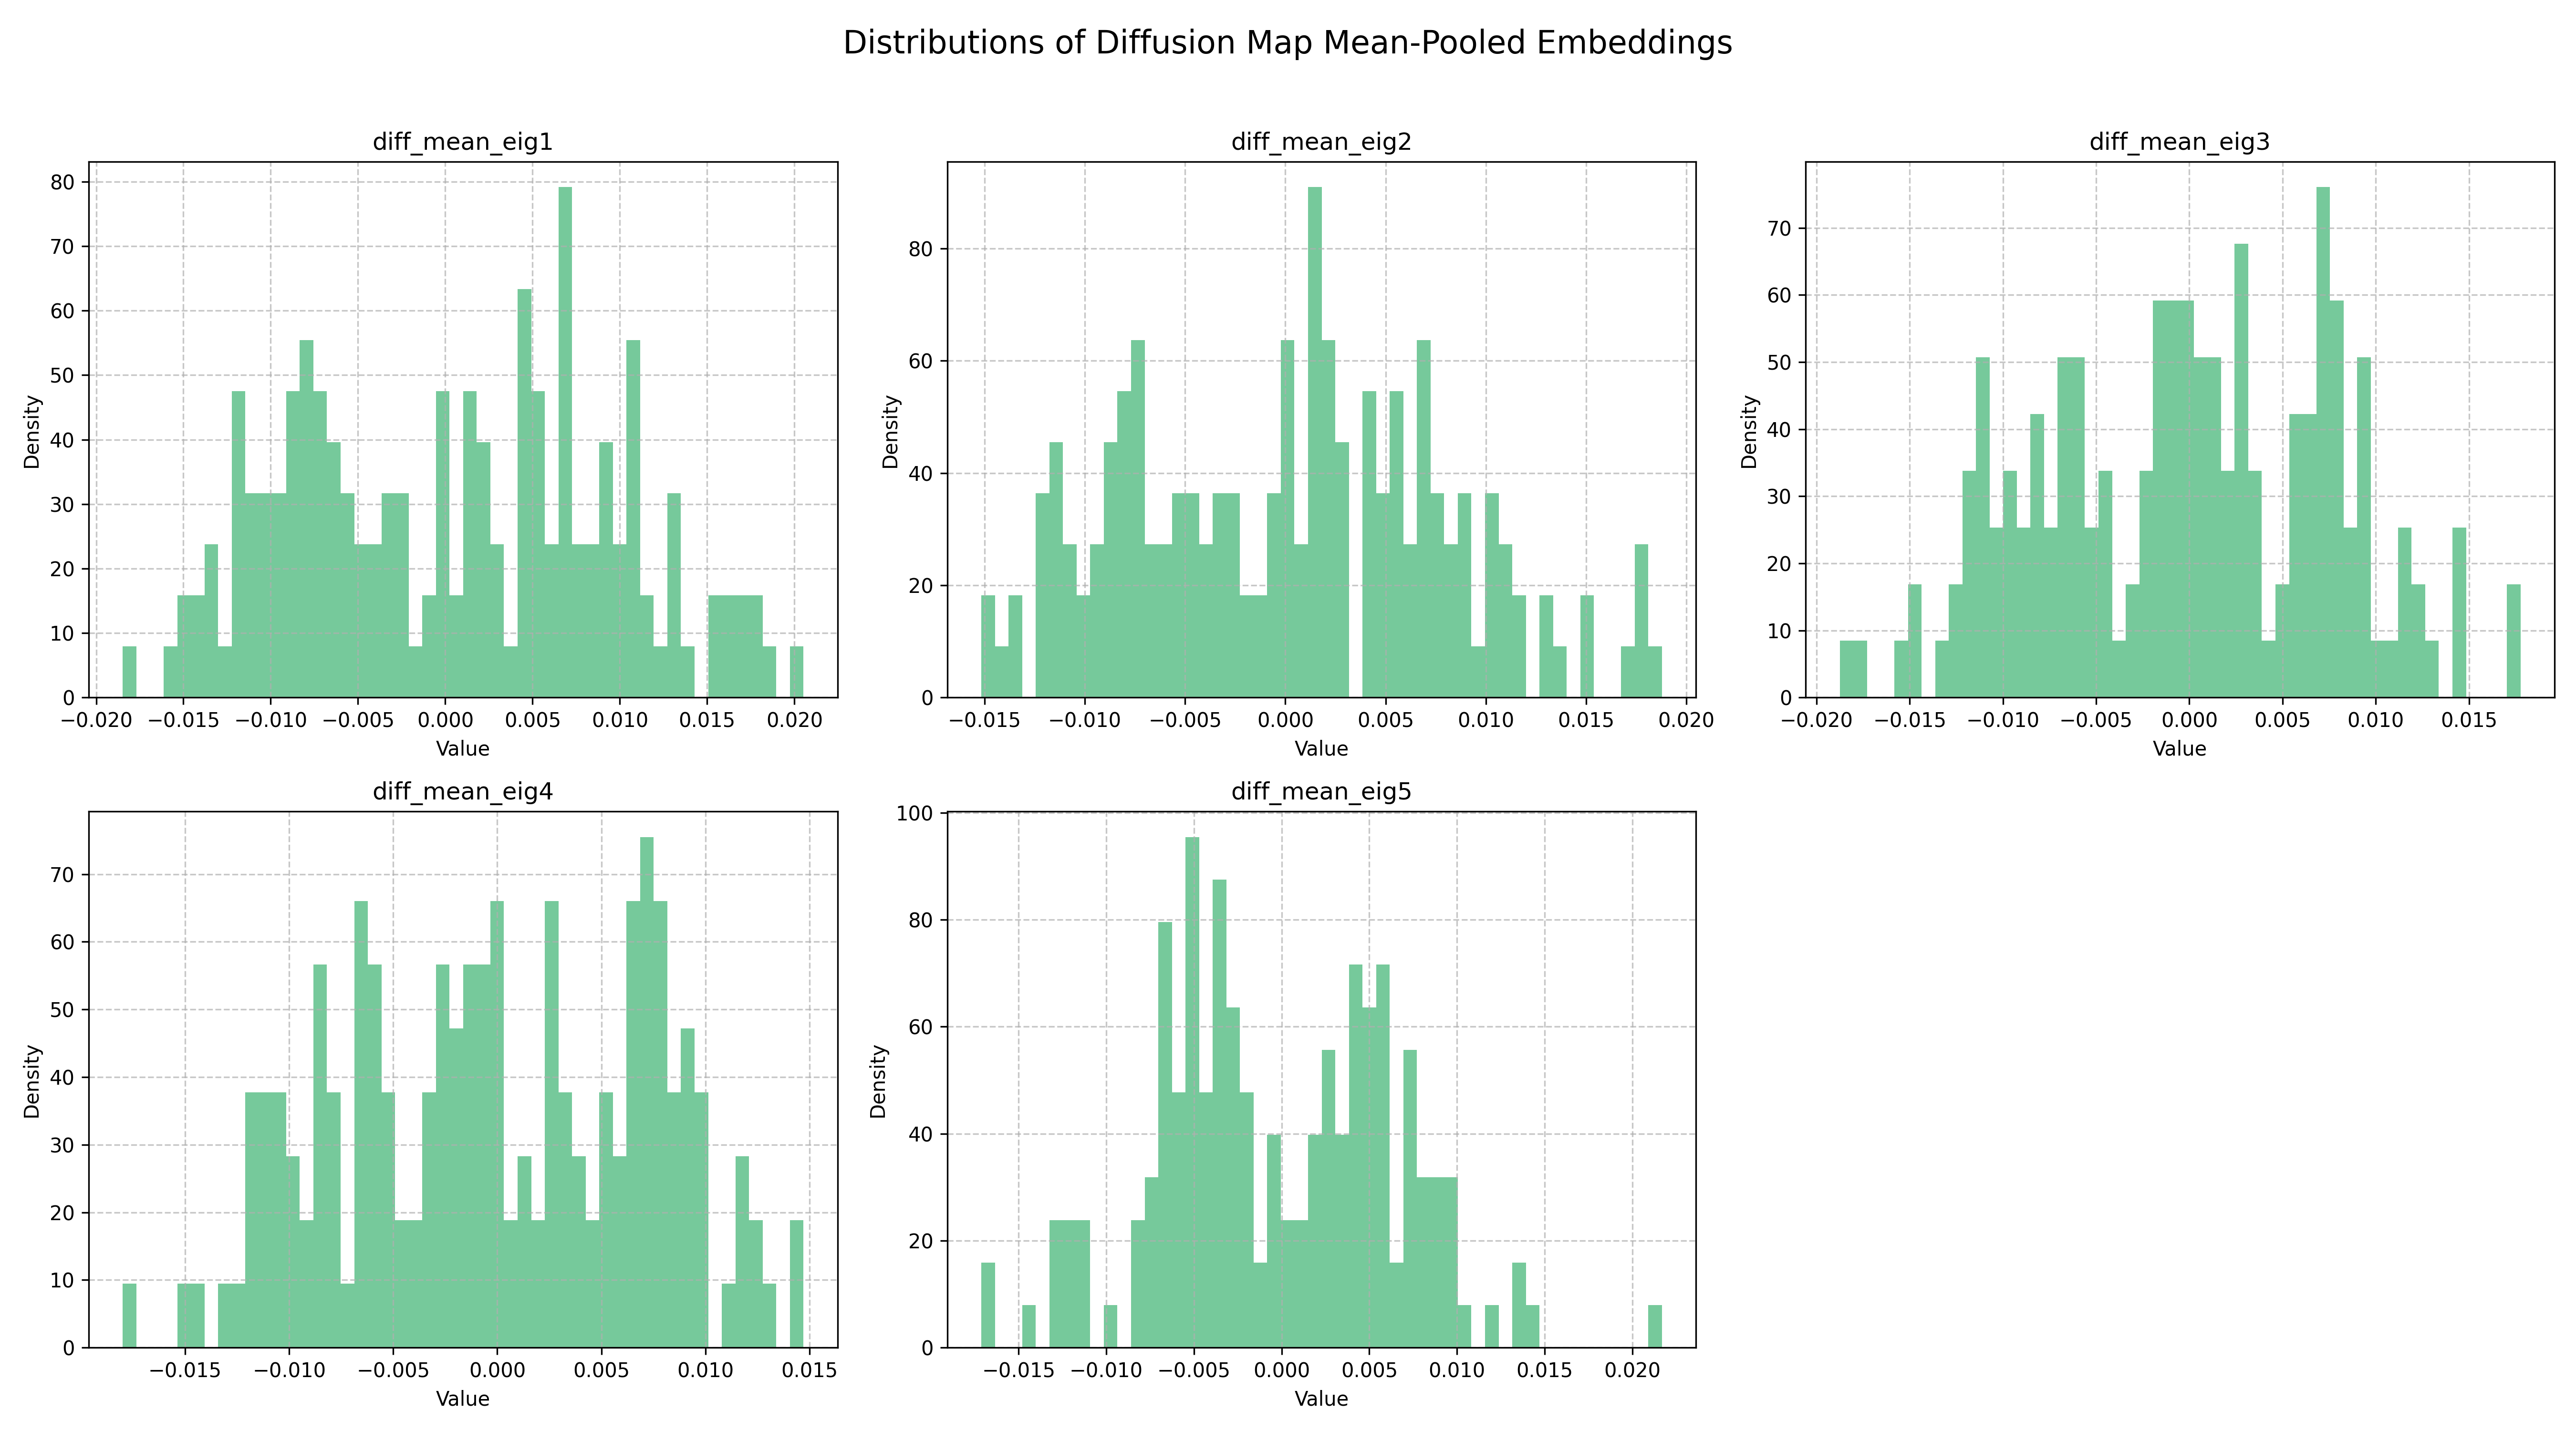
\includegraphics[width=0.5\textwidth]{../input_files/plots/engineered_feature_dist_diff_mean_3_20250527-135752.png}
    \caption{Histograms showing the distributions of the mean-pooled embeddings from the top 5 eigenvectors of the diffusion map. These features, computed on merger trees and imputed for large graphs, were intended to capture structural information, but ultimately failed to predict cosmological parameters.}
    \label{fig:diffusion_feature_dist_mean}
\end{figure}

\begin{figure}[h!]
    \centering
    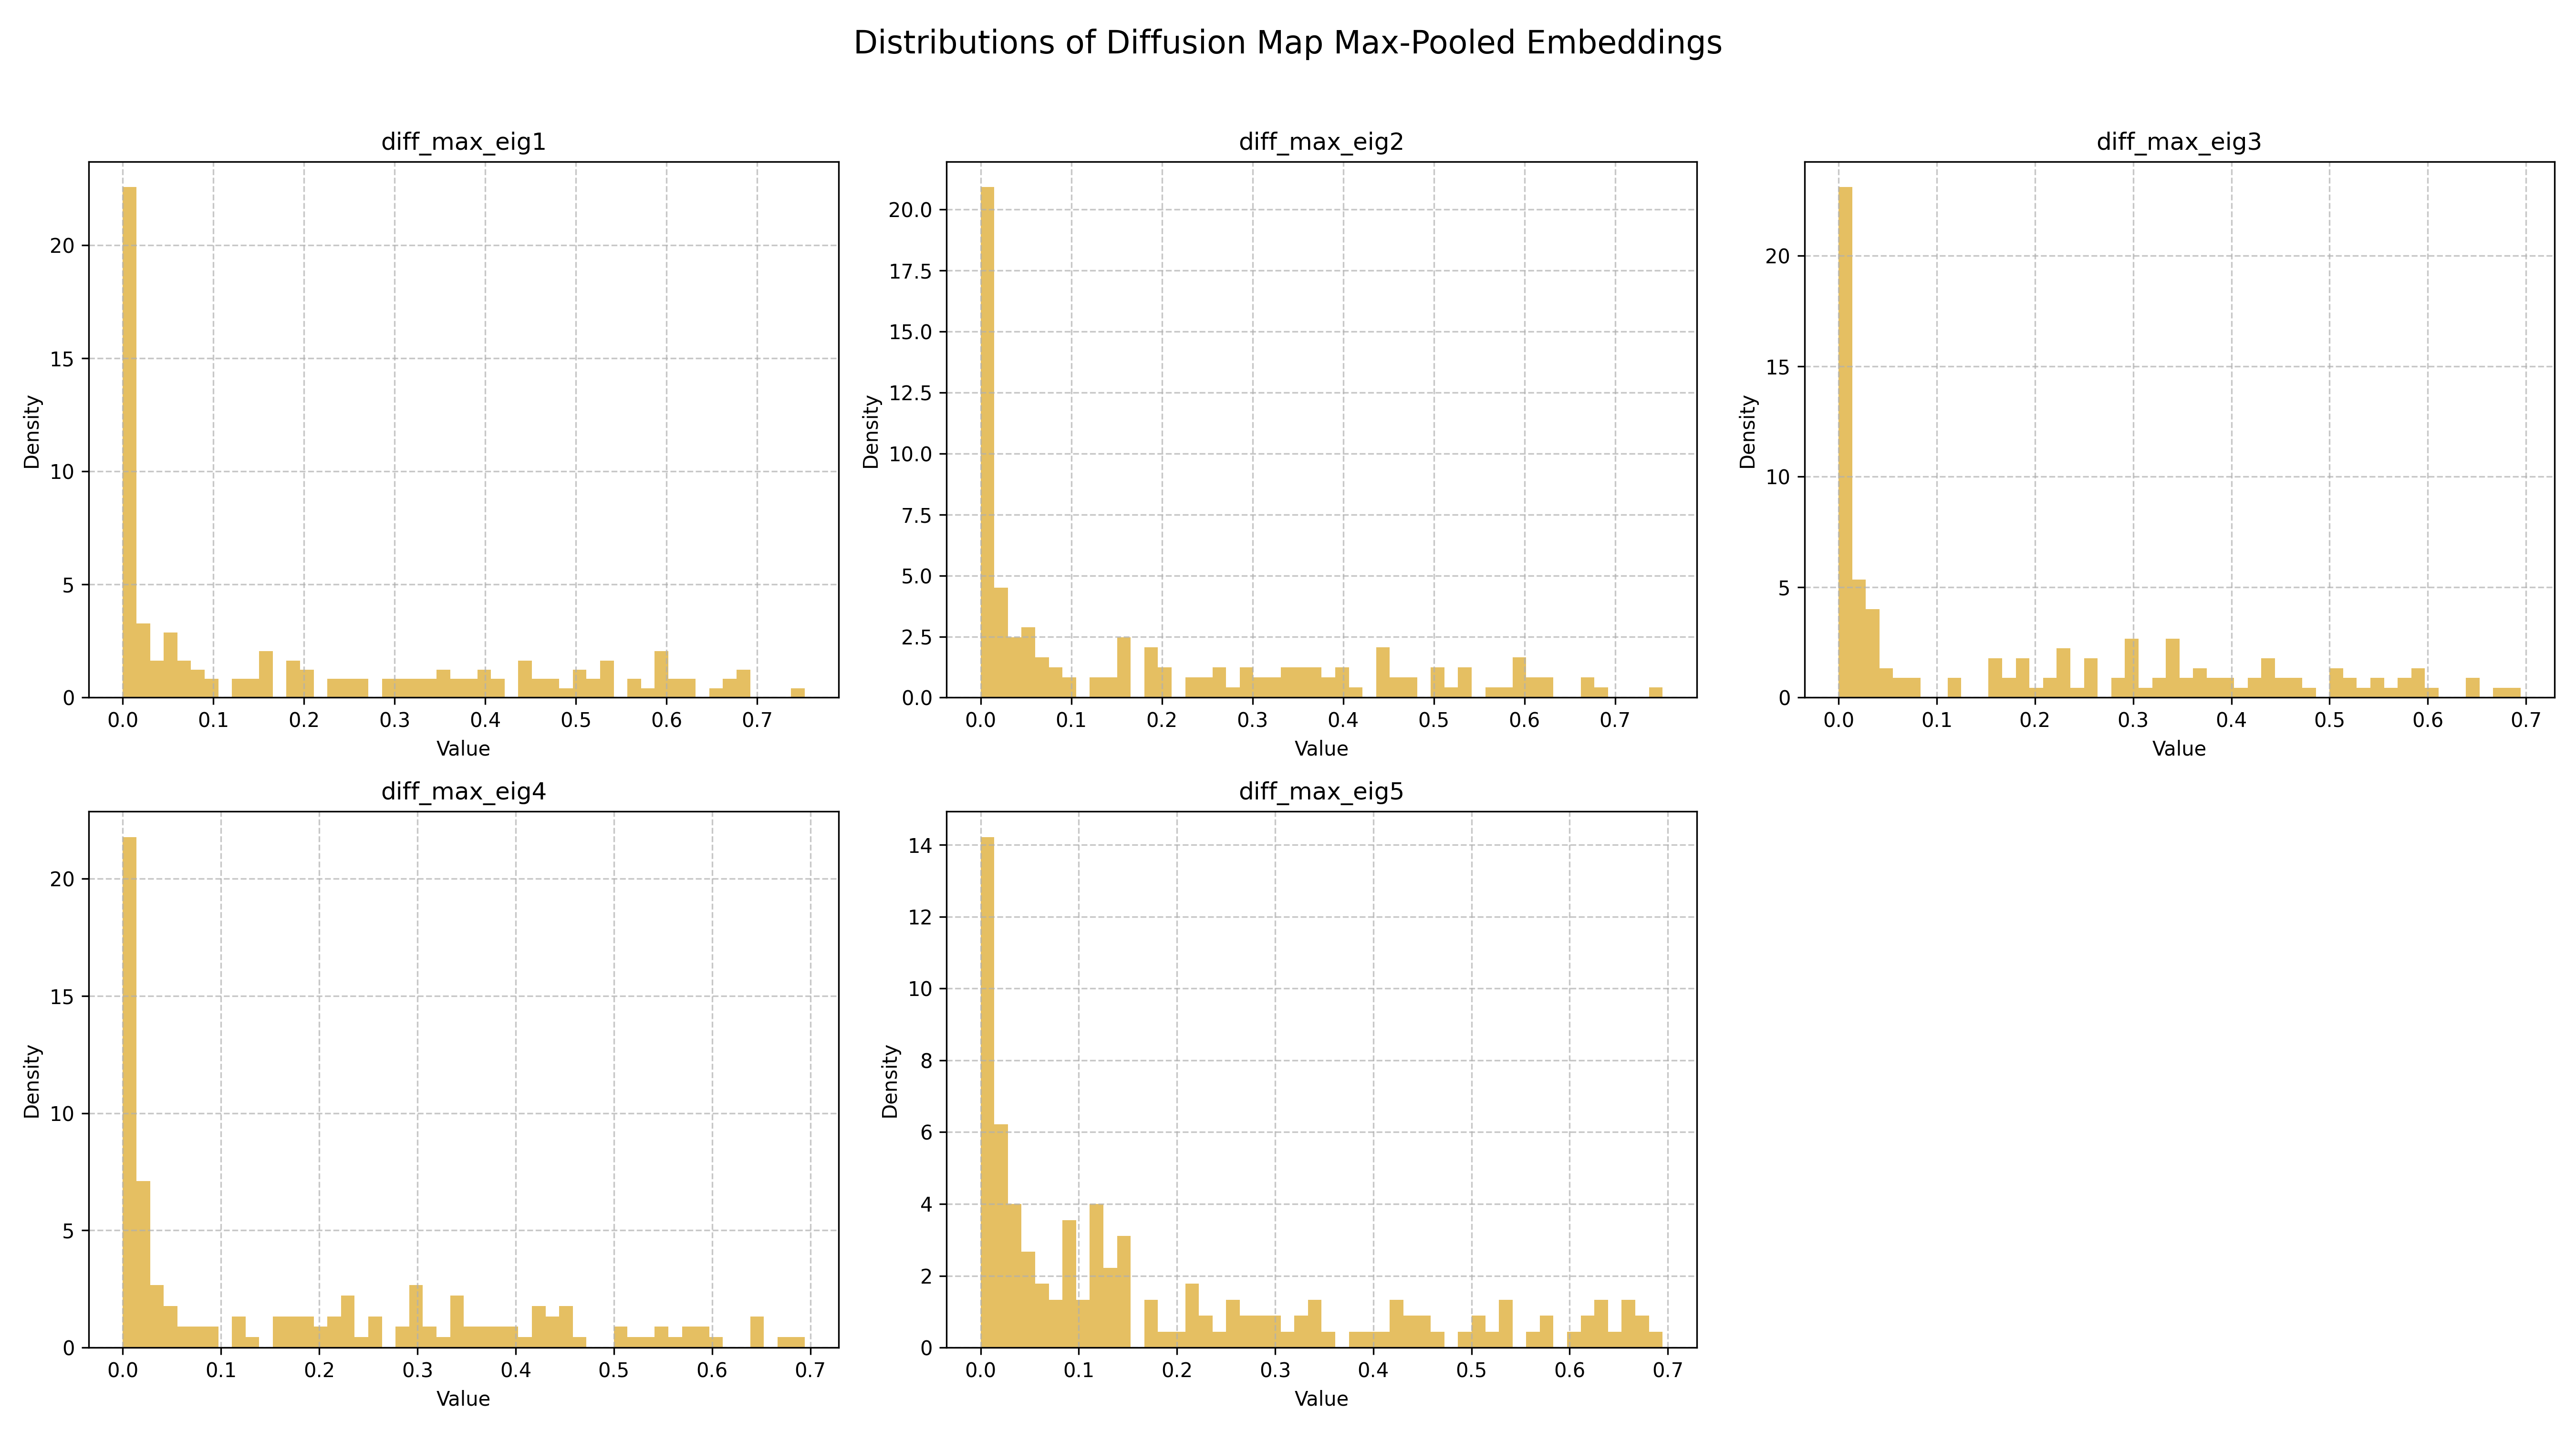
\includegraphics[width=0.5\textwidth]{../input_files/plots/engineered_feature_dist_diff_max_4_20250527-135752.png}
    \caption{Distributions of the max-pooled diffusion map embeddings, showing the feature distributions after mean imputation of NaN values resulting from computational constraints for large graphs. These features did not prove effective in predicting cosmological parameters.}
    \label{fig:diffusion_feature_dist}
\end{figure}

\begin{figure}[h!]
    \centering
    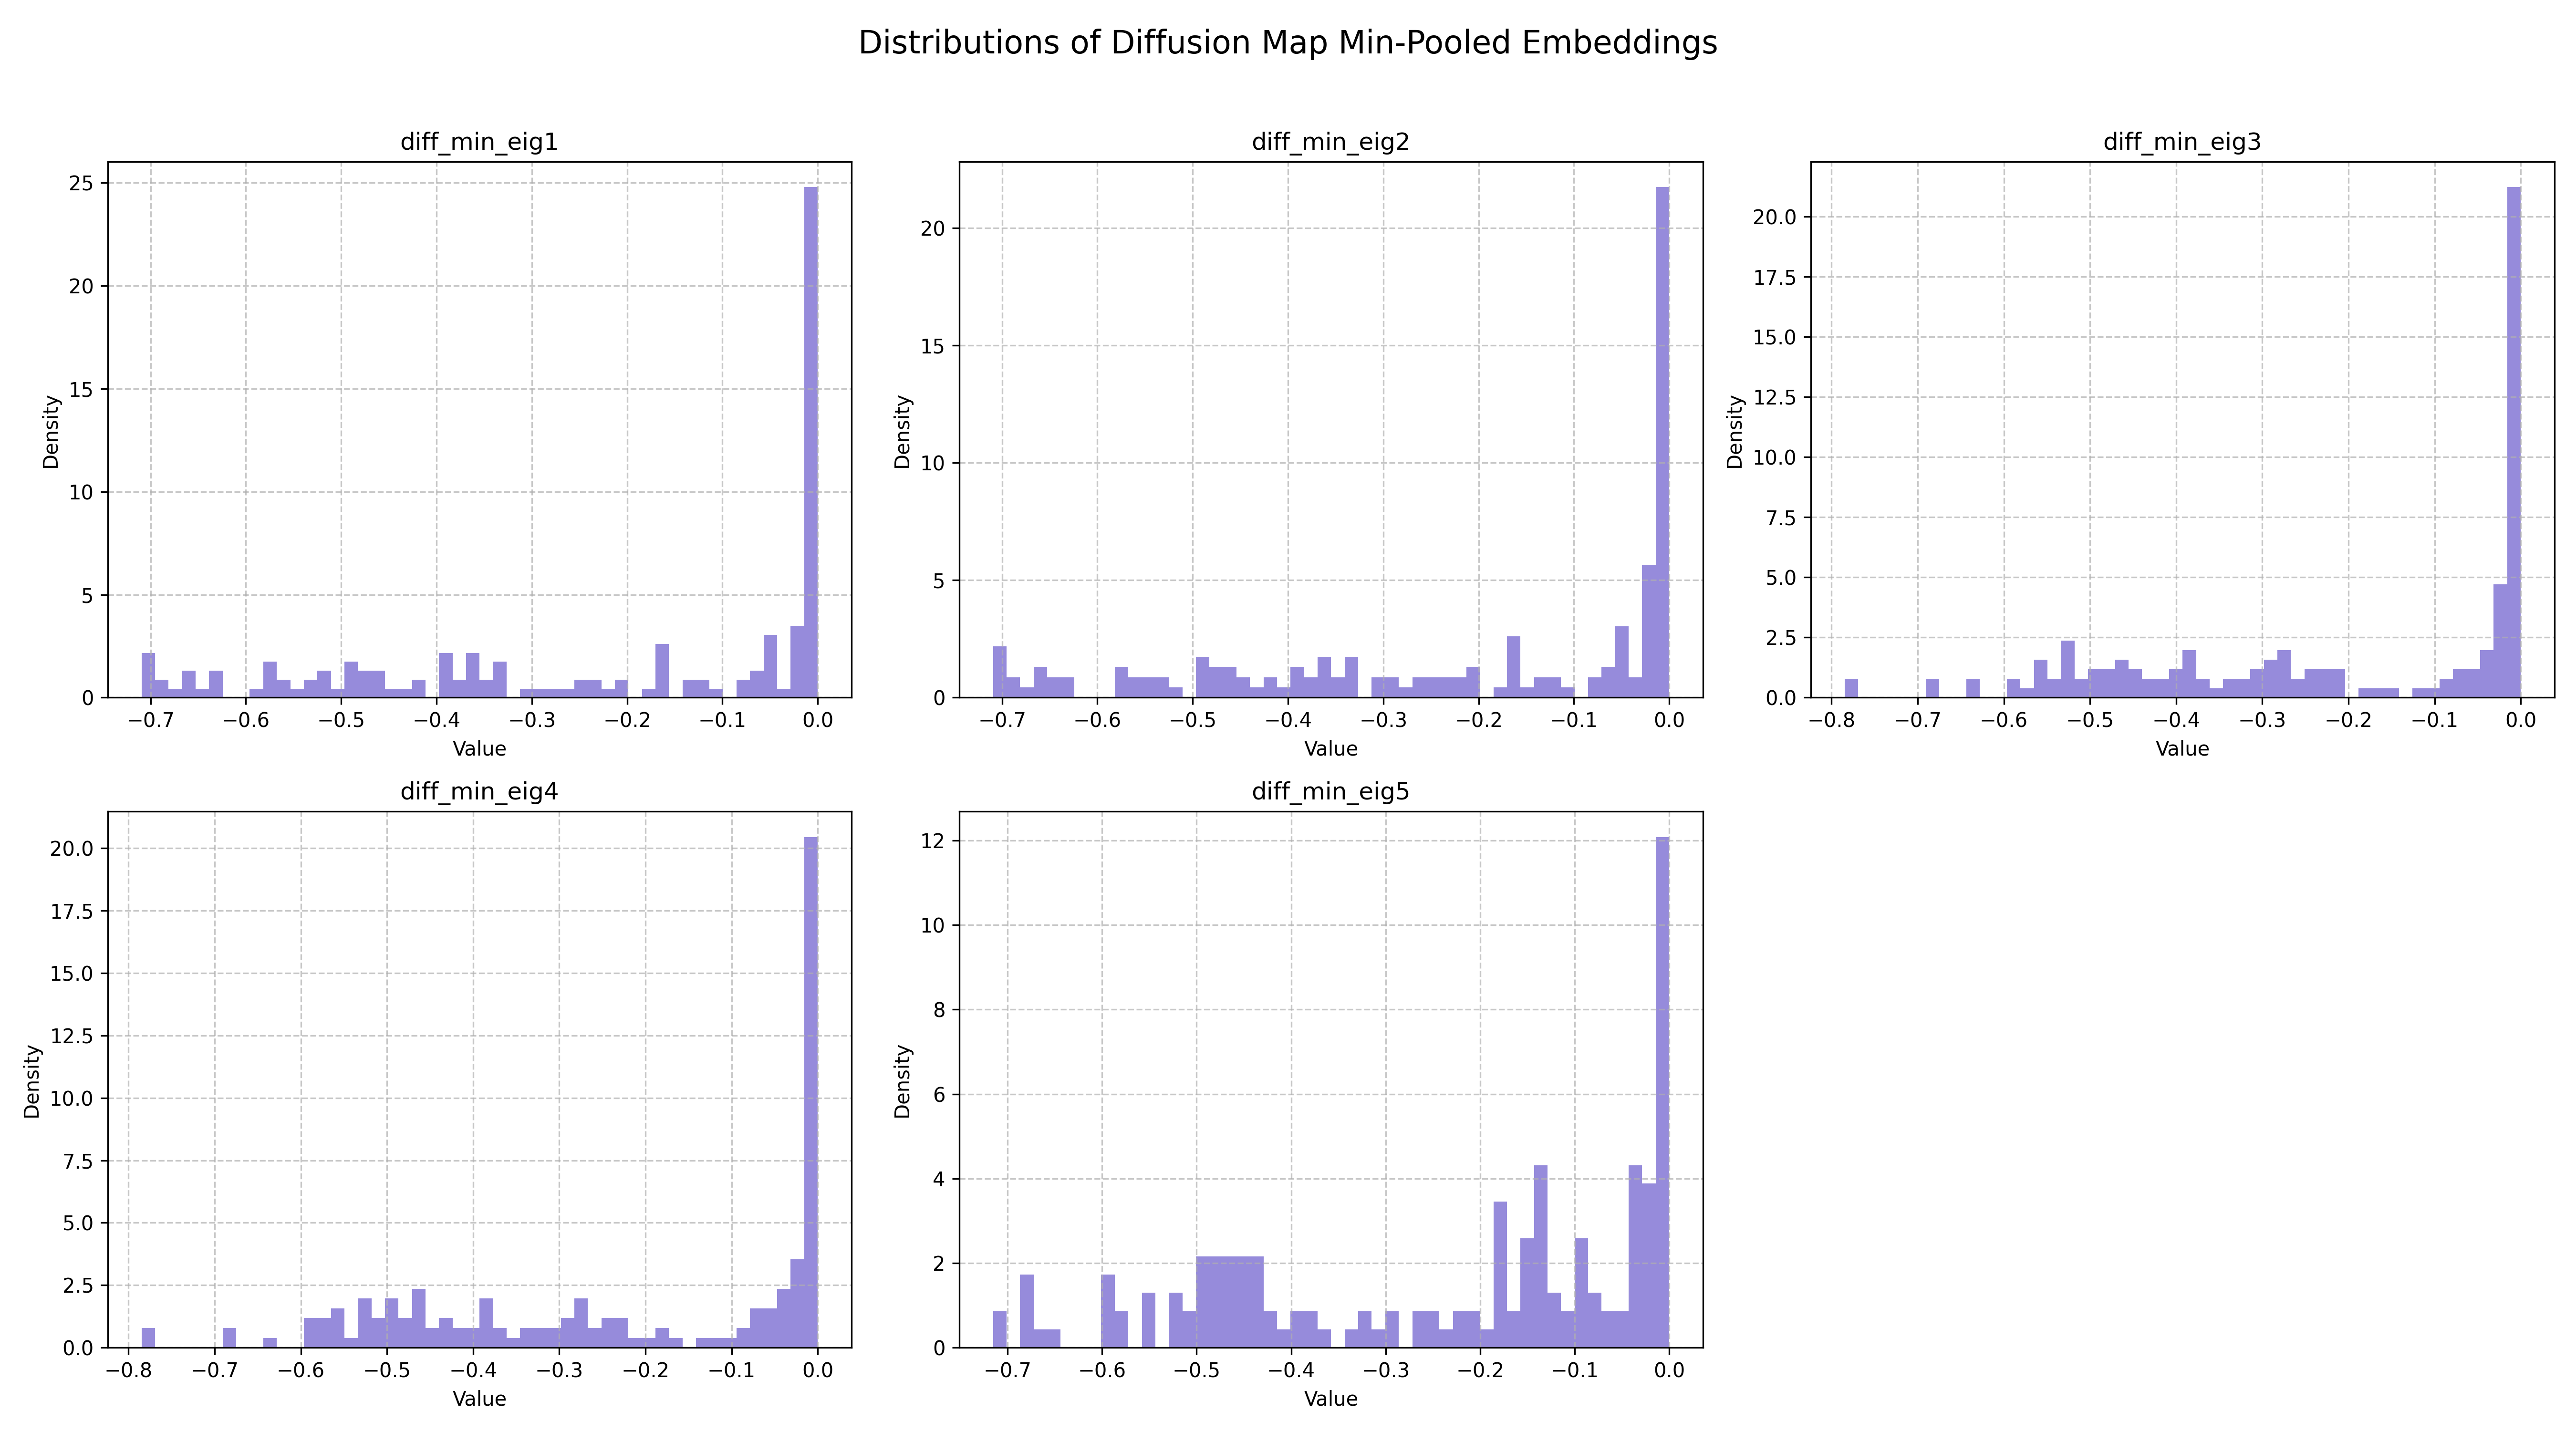
\includegraphics[width=0.5\textwidth]{../input_files/plots/engineered_feature_dist_diff_min_5_20250527-135752.png}
    \caption{Histograms showing the distribution of the minimum-pooled diffusion map embeddings for the first five eigenvectors, illustrating the impact of imputing NaN values due to computational constraints during feature engineering, which likely contributed to the poor performance of these features in predicting cosmological parameters.}
    \label{fig:diffusion_feature_dist_min}
\end{figure}

\subsection{Dimensionality Reduction of Engineered Features}

To reduce dimensionality and decorrelate features, Principal Component Analysis (PCA) was applied to the mean-imputed 24 engineered features derived from the training set. The goal was to retain most of the variance while reducing the number of features. The PCA explained variance plot shown in Figure \ref{fig:pca_explained_variance} shows the cumulative and individual explained variance per component. Based on this analysis, it was determined that 8 principal components were sufficient to explain approximately 96.29\% of the variance in the engineered feature space. Consequently, both training and test engineered feature sets were transformed into this 8-dimensional PCA space.

\begin{figure}[h!]
    \centering
    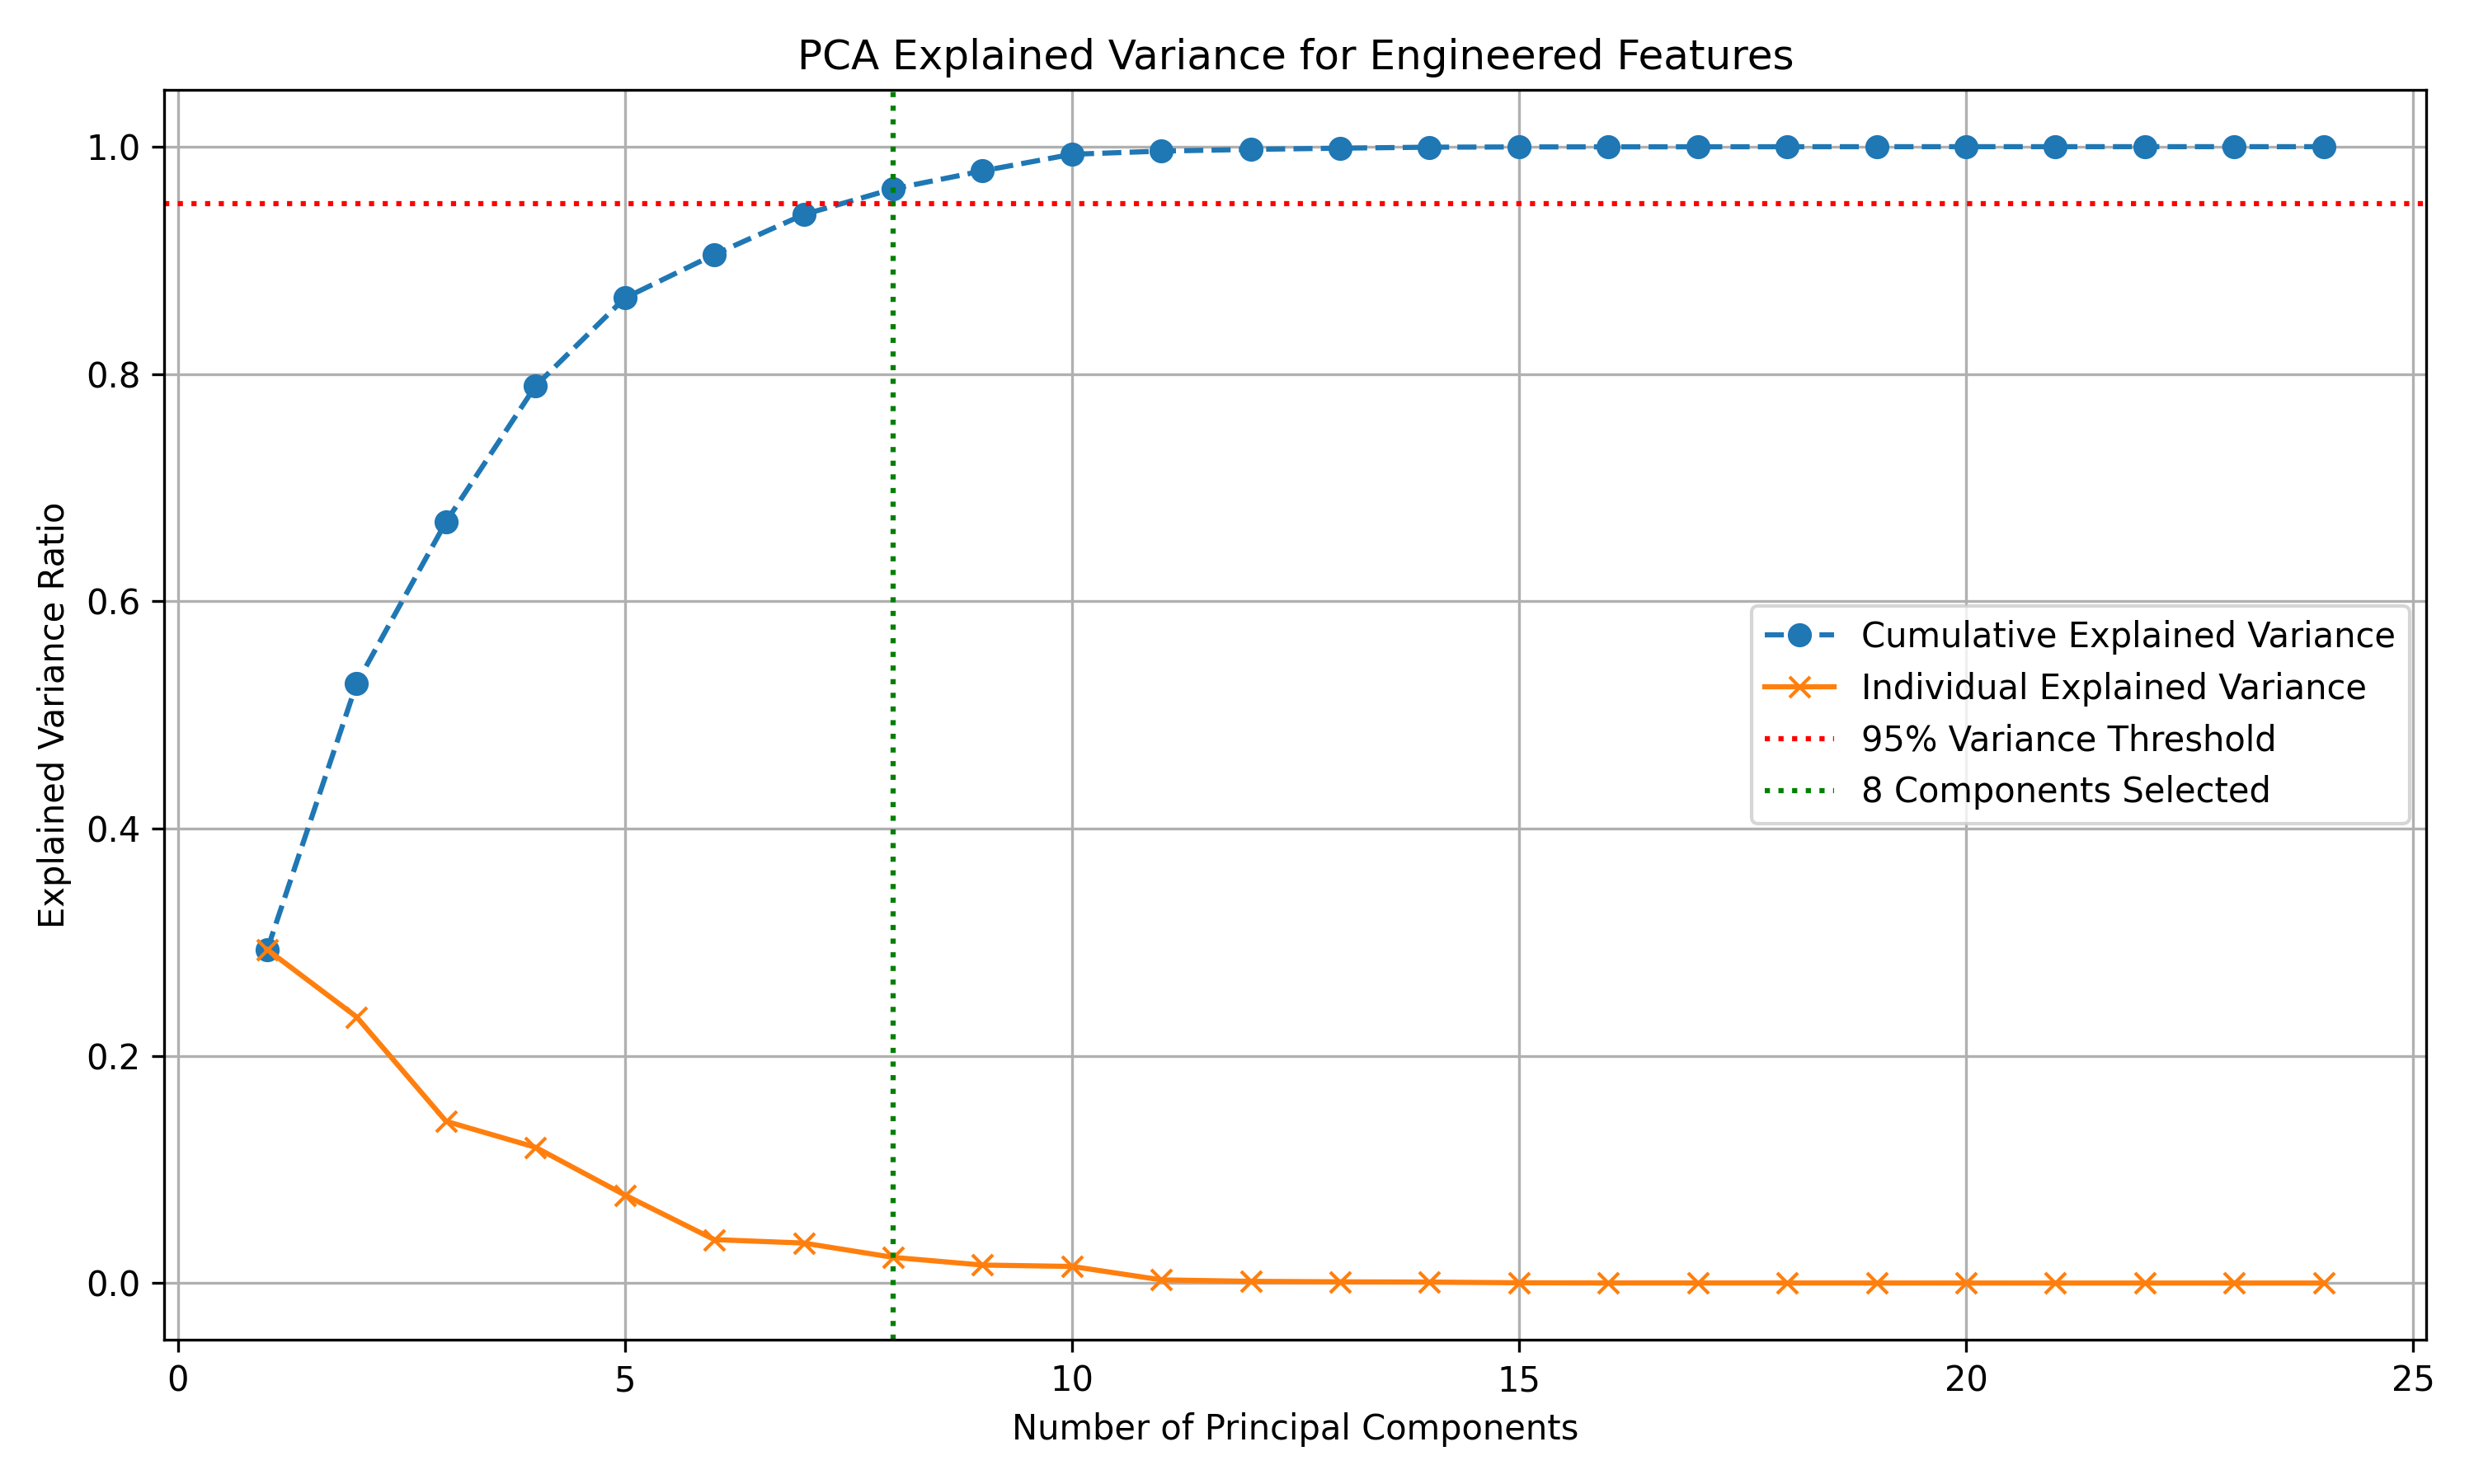
\includegraphics[width=0.5\textwidth]{../input_files/plots/pca_explained_variance_plot_1_20250527-134016.png}
    \caption{PCA explained variance plot for engineered features. Eight principal components were sufficient to explain 96.29\% of the variance. However, models trained on these PCA-transformed features performed poorly, suggesting that the retained variance did not capture information relevant for predicting cosmological parameters.}
    \label{fig:pca_explained_variance}
\end{figure}

To visualize the PCA-transformed data, scatter plots of the first two principal components (PC1 vs. PC2) were generated, colored by the true values of $\Omega_m$ and $\sigma_8$, as shown in Figure \ref{fig:pca_projection}. These projections did not reveal any immediately obvious strong linear separation or clear clustering of data points corresponding to different $\Omega_m$ or $\sigma_8$ values. The points were largely intermingled, suggesting that the first two principal components of the engineered features may not linearly capture strong cosmological signatures in a visually separable manner. This lack of clear visual separation hints that the relationship between the engineered features (even after PCA) and the cosmological parameters might be complex, non-linear, or that these features are not strongly discriminative.

\begin{figure}[h!]
    \centering
    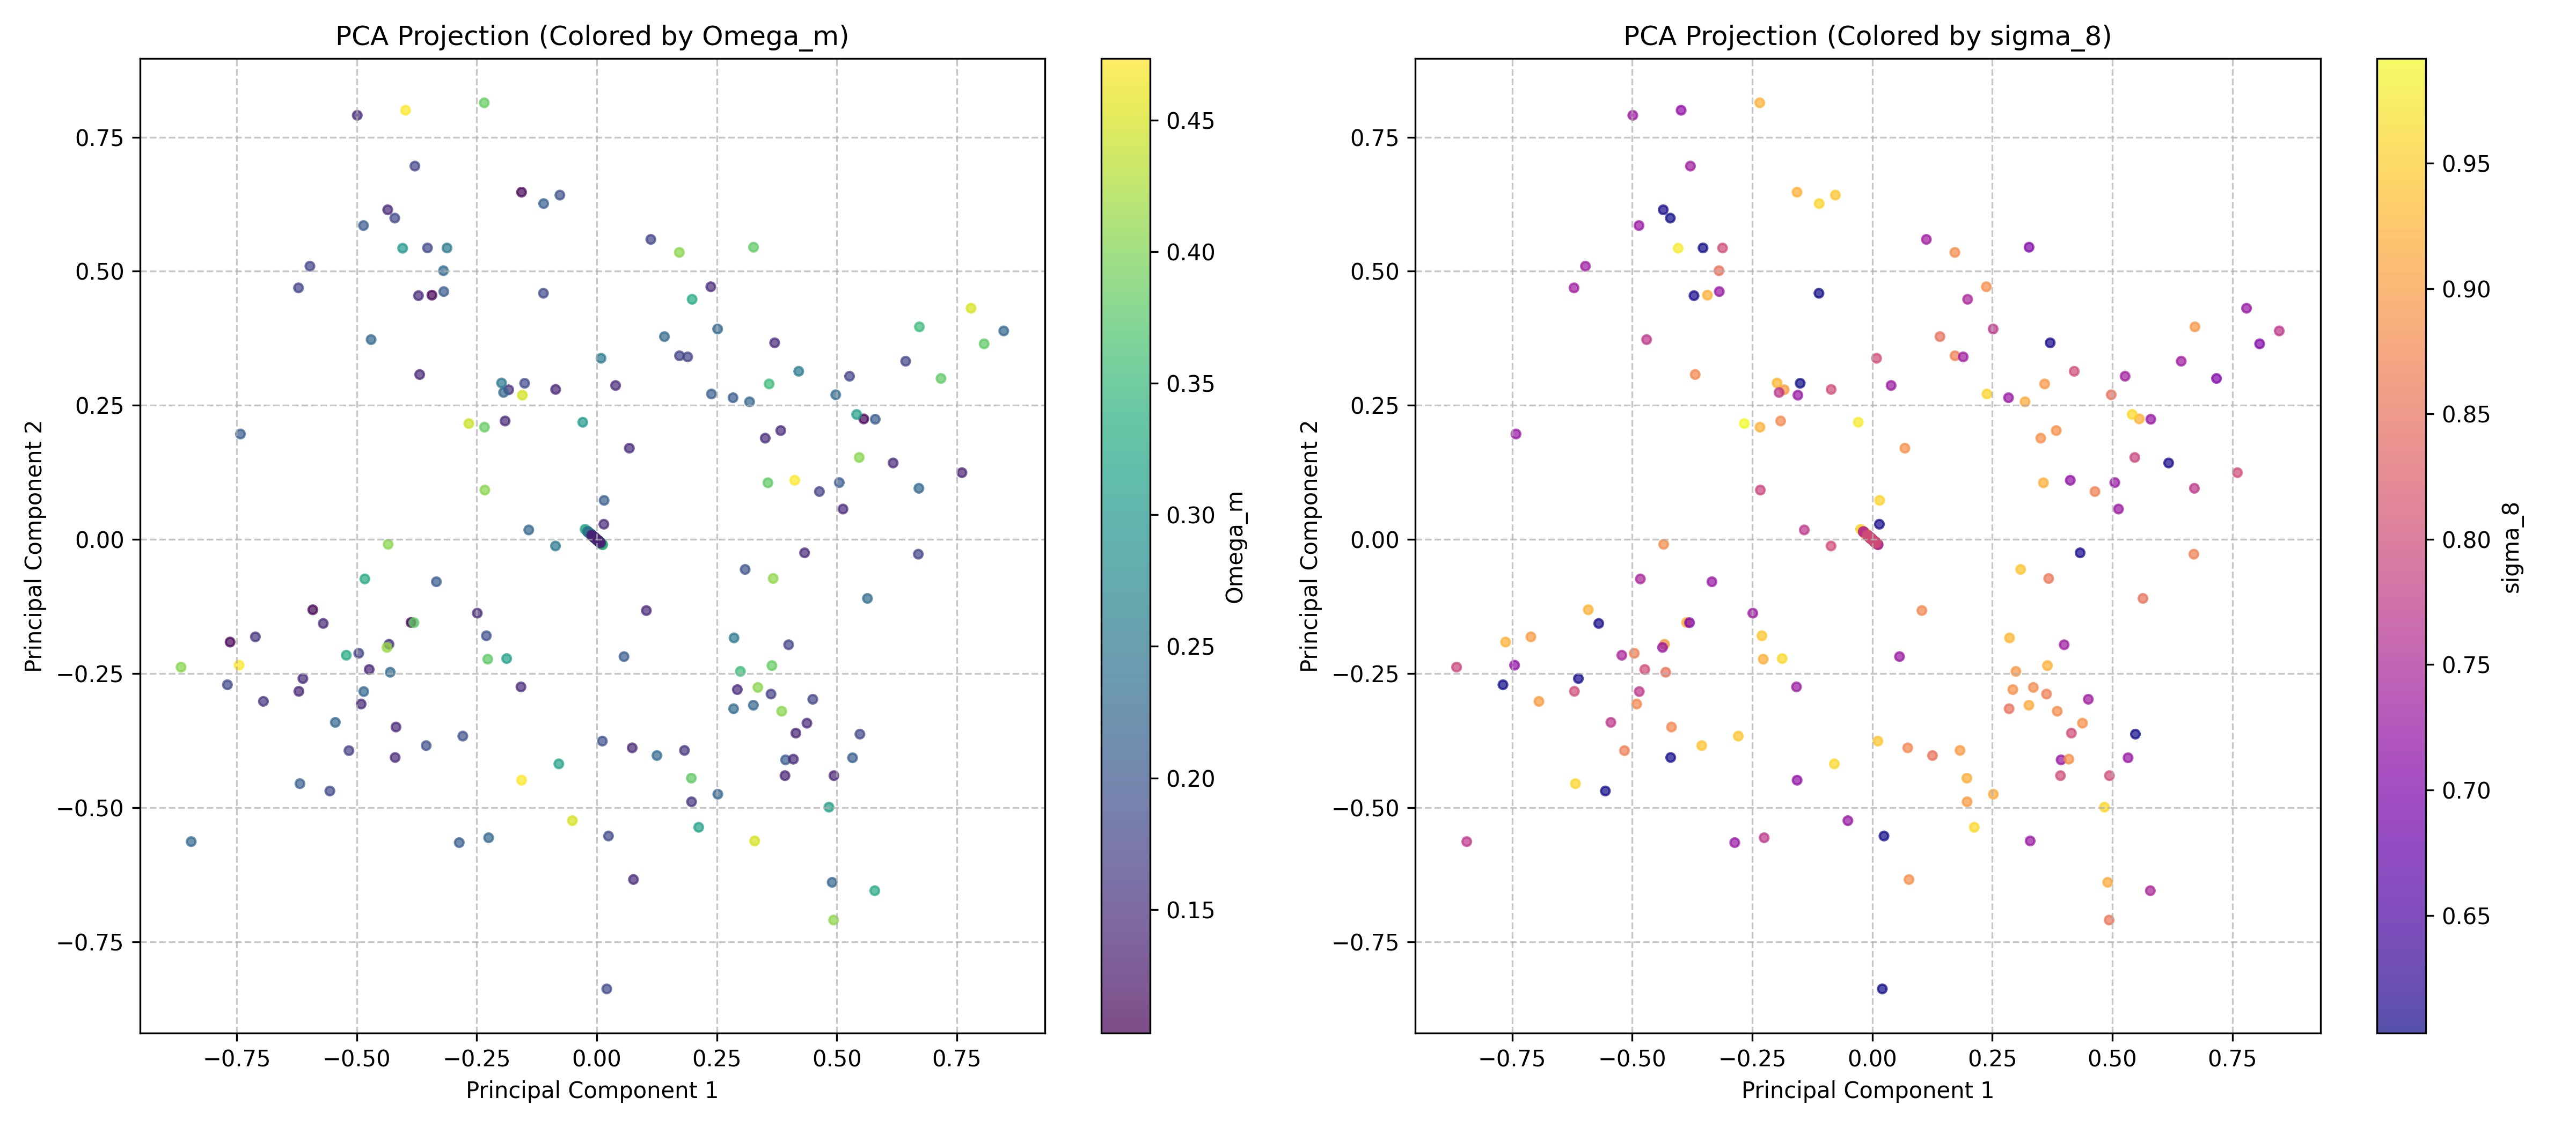
\includegraphics[width=0.5\textwidth]{../input_files/plots/pca_projection_plot_6_20250527-135752.png}
    \caption{Scatter plots of the first two principal components of the engineered features, colored by $\Omega_m$ (left) and $\sigma_8$ (right). There is no clear visual separation between different values of the cosmological parameters.}
    \label{fig:pca_projection}
\end{figure}

\subsection{Baseline Feature Sets}

Two baseline approaches were established for comparison:
\begin{enumerate}
    \item Baseline Aggregated Node Features: For each graph, 16 features were computed by taking the mean, standard deviation, minimum, and maximum of each of the 4 normalized node features across all nodes in that graph. These features provide simple global statistics of the halo properties within each merger tree. No NaNs were present in these baseline features after computation.
    \item Graph Convolutional Network (GCN): A GCN model was implemented for graph-level regression. It consisted of two `GCNConv` layers with ReLU activations, followed by a global mean pooling layer and two fully connected layers for regression. The GCN was trained on normalized node features and graph structures for 50 epochs on a CPU.
\end{enumerate}

\subsection{Predictive Performance of Cosmological Parameters}

Regression models (Random Forest Regressor - RFR, Gradient Boosting Regressor - GBR) were trained on both the PCA-transformed engineered features and the baseline aggregated node features. The GCN provided a deep learning baseline. Performance was evaluated using R-squared (R²) and Mean Squared Error (MSE) on the test set. All hyperparameters for RFR and GBR were tuned using `GridSearchCV` with `GroupKFold` (5 splits) based on `lh\_id` to prevent data leakage.

A summary of the model performances is presented in Table \ref{tab:model_performance}. The visualizations of the performance comparison are shown in Figure \ref{fig:model_performance_r2} for R² and Figure \ref{fig:model_performance_mse} for MSE.

\begin{table}[h!]
\centering
\caption{Model Performance on Test Set for Predicting $\Omega_m$ and $\sigma_8$}
\begin{tabular}{|l|l|l|l|l|}
\hline
Feature Set             & Model & Target    & R²      & MSE        \\ \hline
Engineered + PCA    & RFR   & $\Omega_m$  & -0.2682 & 0.010926   \\ \hline
                        & GBR   & $\Omega_m$  & -0.1885 & 0.010240   \\ \hline
                        & RFR   & $\sigma_8$  & -0.4622 & 0.016500   \\ \hline
                        & GBR   & $\sigma_8$  & -0.4412 & 0.016262   \\ \hline
Baseline Aggregated & RFR   & $\Omega_m$  & 0.8879  & 0.000966   \\ \hline
                        & GBR   & $\Omega_m$  & 0.9134  & 0.000746   \\ \hline
                        & RFR   & $\sigma_8$  & 0.2827  & 0.008094   \\ \hline
                        & GBR   & $\sigma_8$  & 0.4238  & 0.006502   \\ \hline
GCN                     & GCN   & $\Omega_m$  & 0.9786  & 0.000185   \\ \hline
                        & GCN   & $\sigma_8$  & 0.4977  & 0.005668   \\ \hline
\end{tabular}
\label{tab:model_performance}
\end{table}

\begin{figure}[h!]
    \centering
    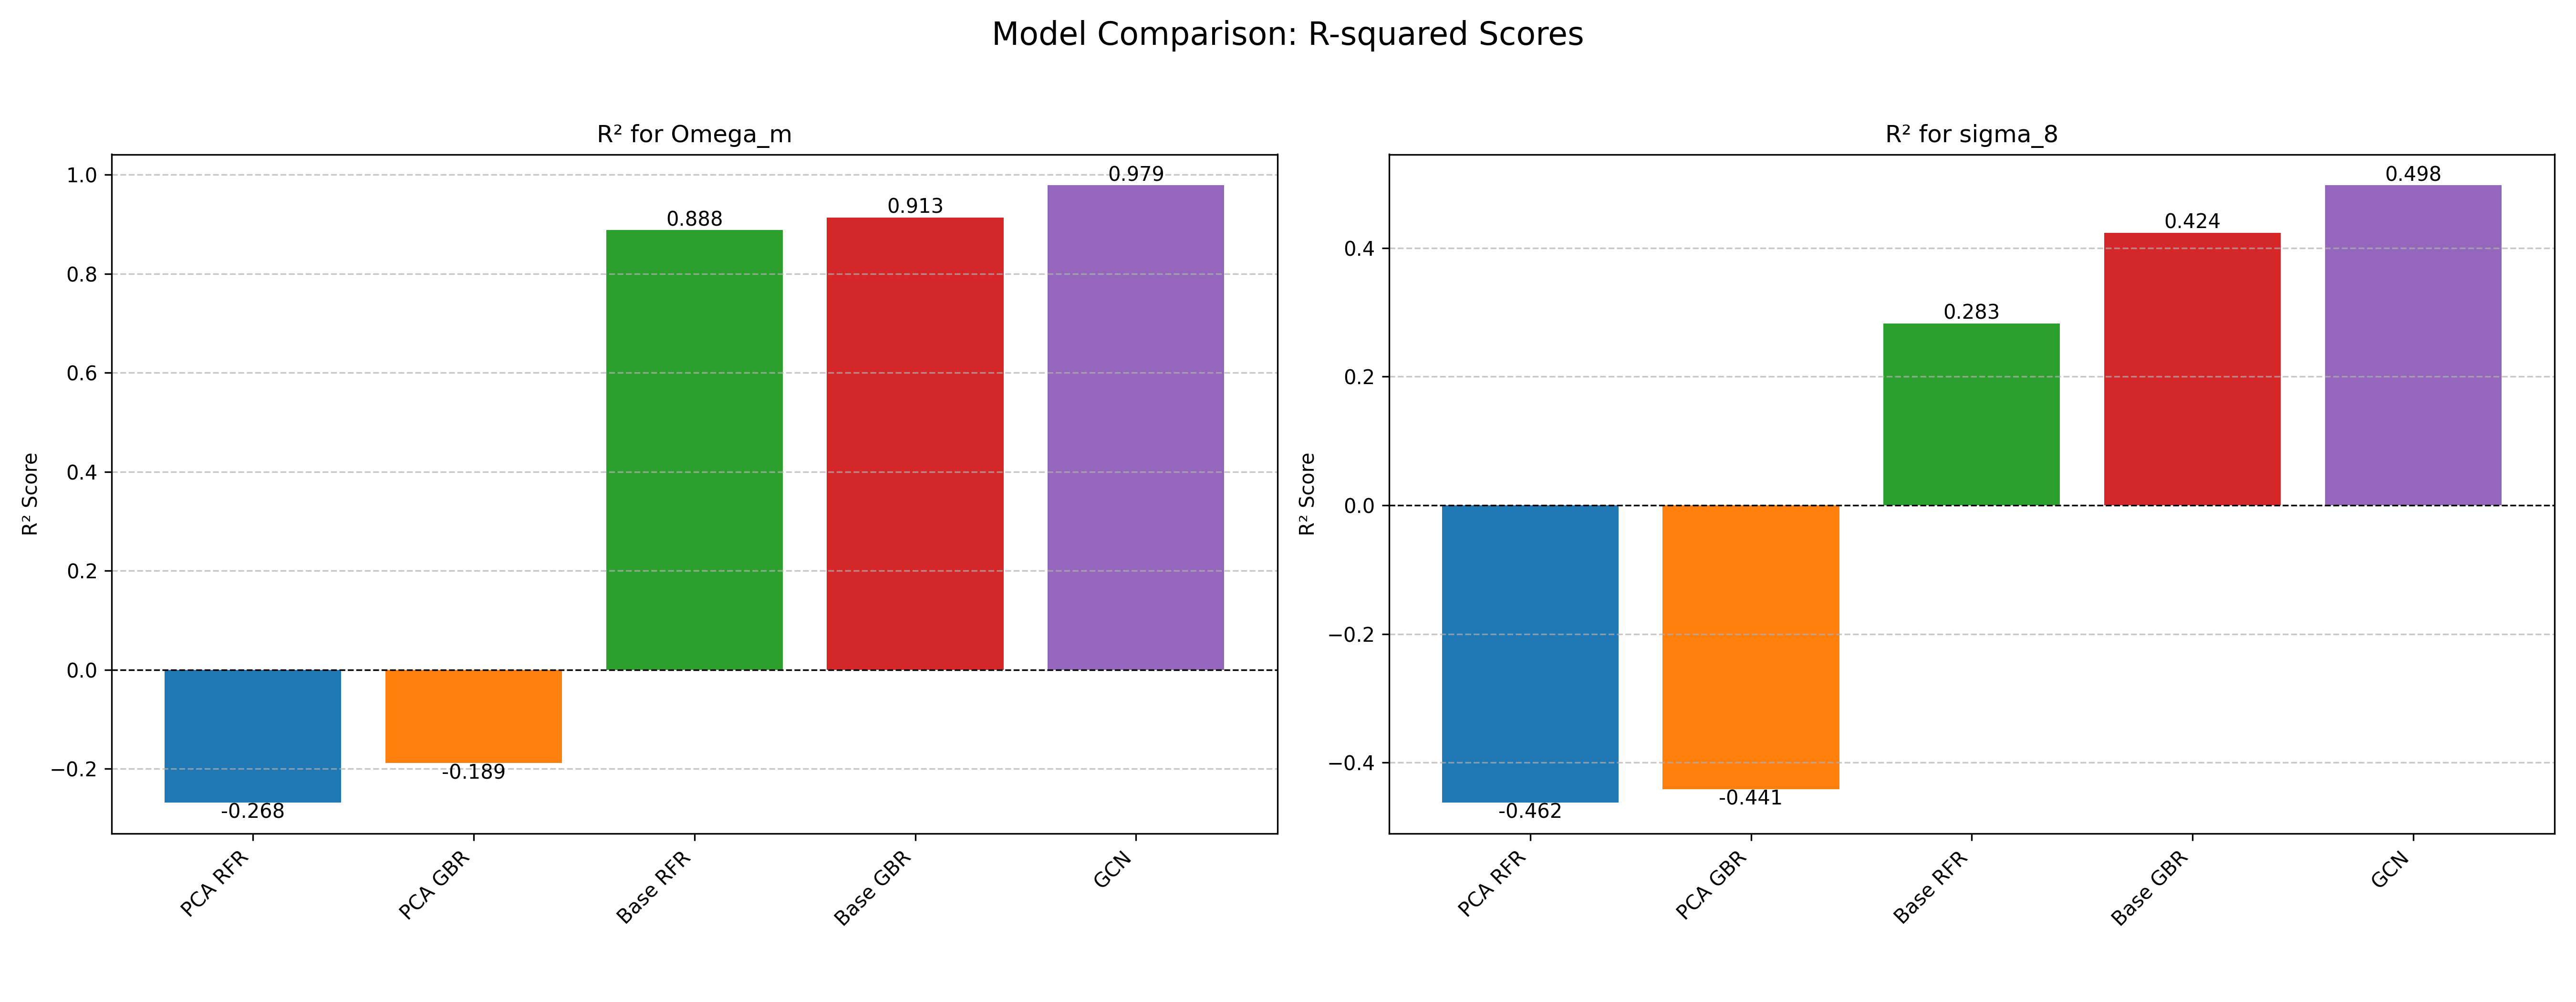
\includegraphics[width=0.5\textwidth]{../input_files/plots/model_performance_r2_11_20250527-135752.png}
    \caption{Comparison of R-squared (R²) scores for predicting $\Omega_m$ and $\sigma_8$ using different feature sets and models. The GCN and baseline aggregated node features outperform engineered features with PCA, which show negative R² values, indicating poor performance.}
    \label{fig:model_performance_r2}
\end{figure}

\begin{figure}[h!]
    \centering
    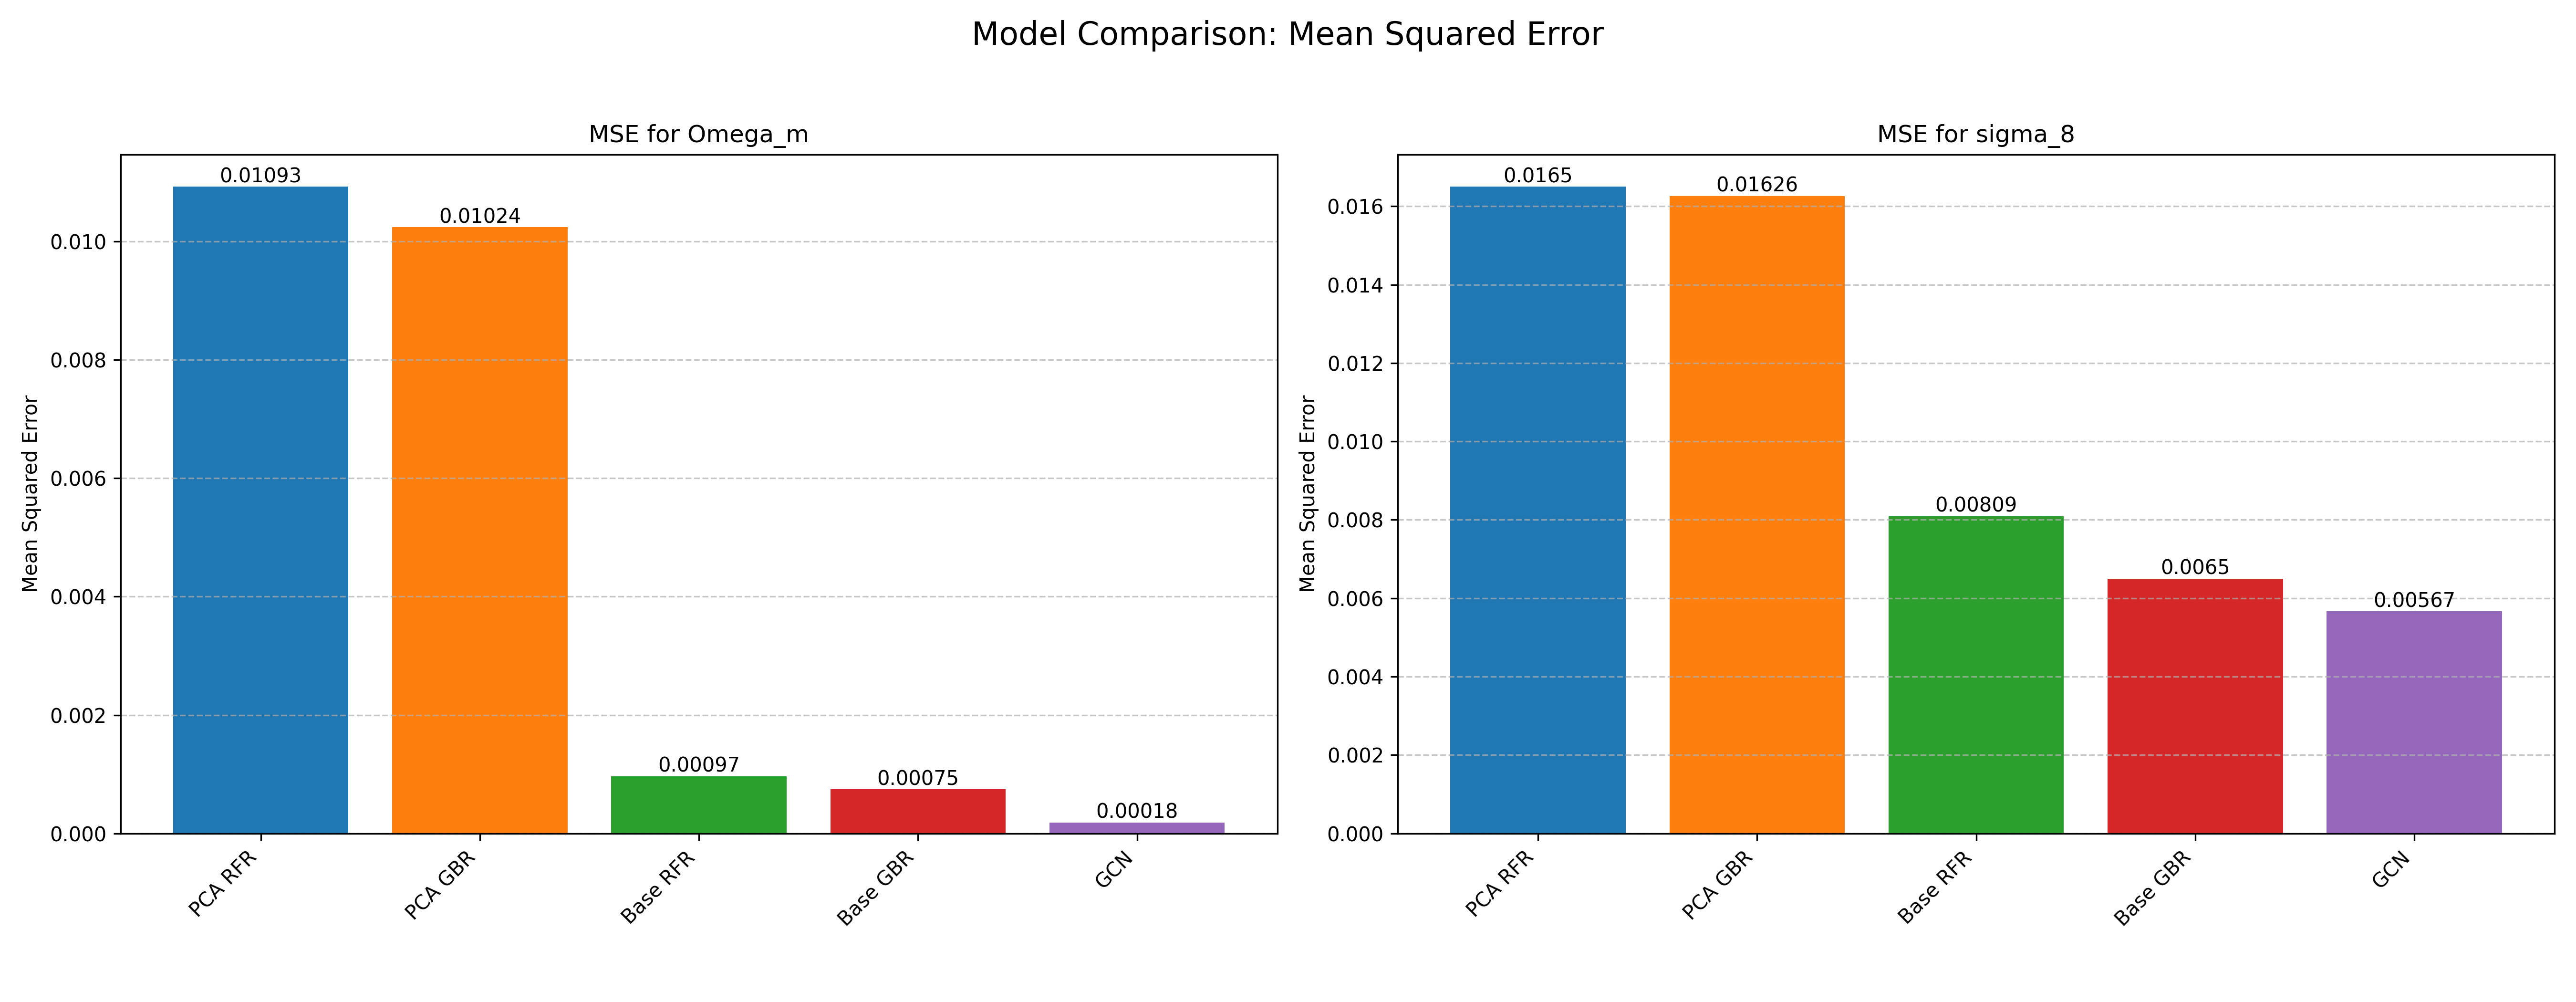
\includegraphics[width=0.5\textwidth]{../input_files/plots/model_performance_mse_12_20250527-135752.png}
    \caption{Mean Squared Error (MSE) comparison of different models (PCA-transformed engineered features with Random Forest Regressor (RFR) and Gradient Boosting Regressor (GBR), baseline aggregated node features with RFR and GBR, and Graph Convolutional Network (GCN)) for predicting $\Omega_m$ and $\sigma_8$. The baseline aggregated node features and the GCN model significantly outperform the engineered features after PCA.}
    \label{fig:model_performance_mse}
\end{figure}

\subsubsection{Prediction of $\Omega_m$}
The GCN model achieved the highest performance, with an R² of 0.9786 and an MSE of 0.000185. This indicates a very strong predictive capability for $\Omega_m$. The Baseline Aggregated Node Features also performed remarkably well. The GBR model yielded an R² of 0.9134 (MSE=0.000746), and the RFR model achieved an R² of 0.8879 (MSE=0.000966). In contrast, the Engineered Features with PCA performed very poorly. Both RFR (R²=-0.2682) and GBR (R²=-0.1885) resulted in negative R² values, indicating that the models performed worse than a horizontal line (predicting the mean). This suggests that these features, in their current form and after PCA, do not capture meaningful information for $\Omega_m$ prediction, or the information is obscured. The differences in performance are also visually apparent in Figure \ref{fig:predicted_vs_true_omega_m}.

\subsubsection{Prediction of $\sigma_8$}
The GCN model again showed the best performance for $\sigma_8$, with an R² of 0.4977 and an MSE of 0.005668. While this is a positive R², it is considerably lower than for $\Omega_m$, suggesting $\sigma_8$ is harder to predict from merger tree morphology. The Baseline Aggregated Node Features with GBR achieved an R² of 0.4238 (MSE=0.006502), and with RFR an R² of 0.2827 (MSE=0.008094). These results are modest but significantly better than the engineered features. The Engineered Features with PCA again failed to provide predictive power for $\sigma_8$, with RFR (R²=-0.4622) and GBR (R²=-0.4412) yielding negative R² values. These results are visually summarized in Figure \ref{fig:predicted_vs_true_sigma_8}.

\begin{figure}[h!]
    \centering
    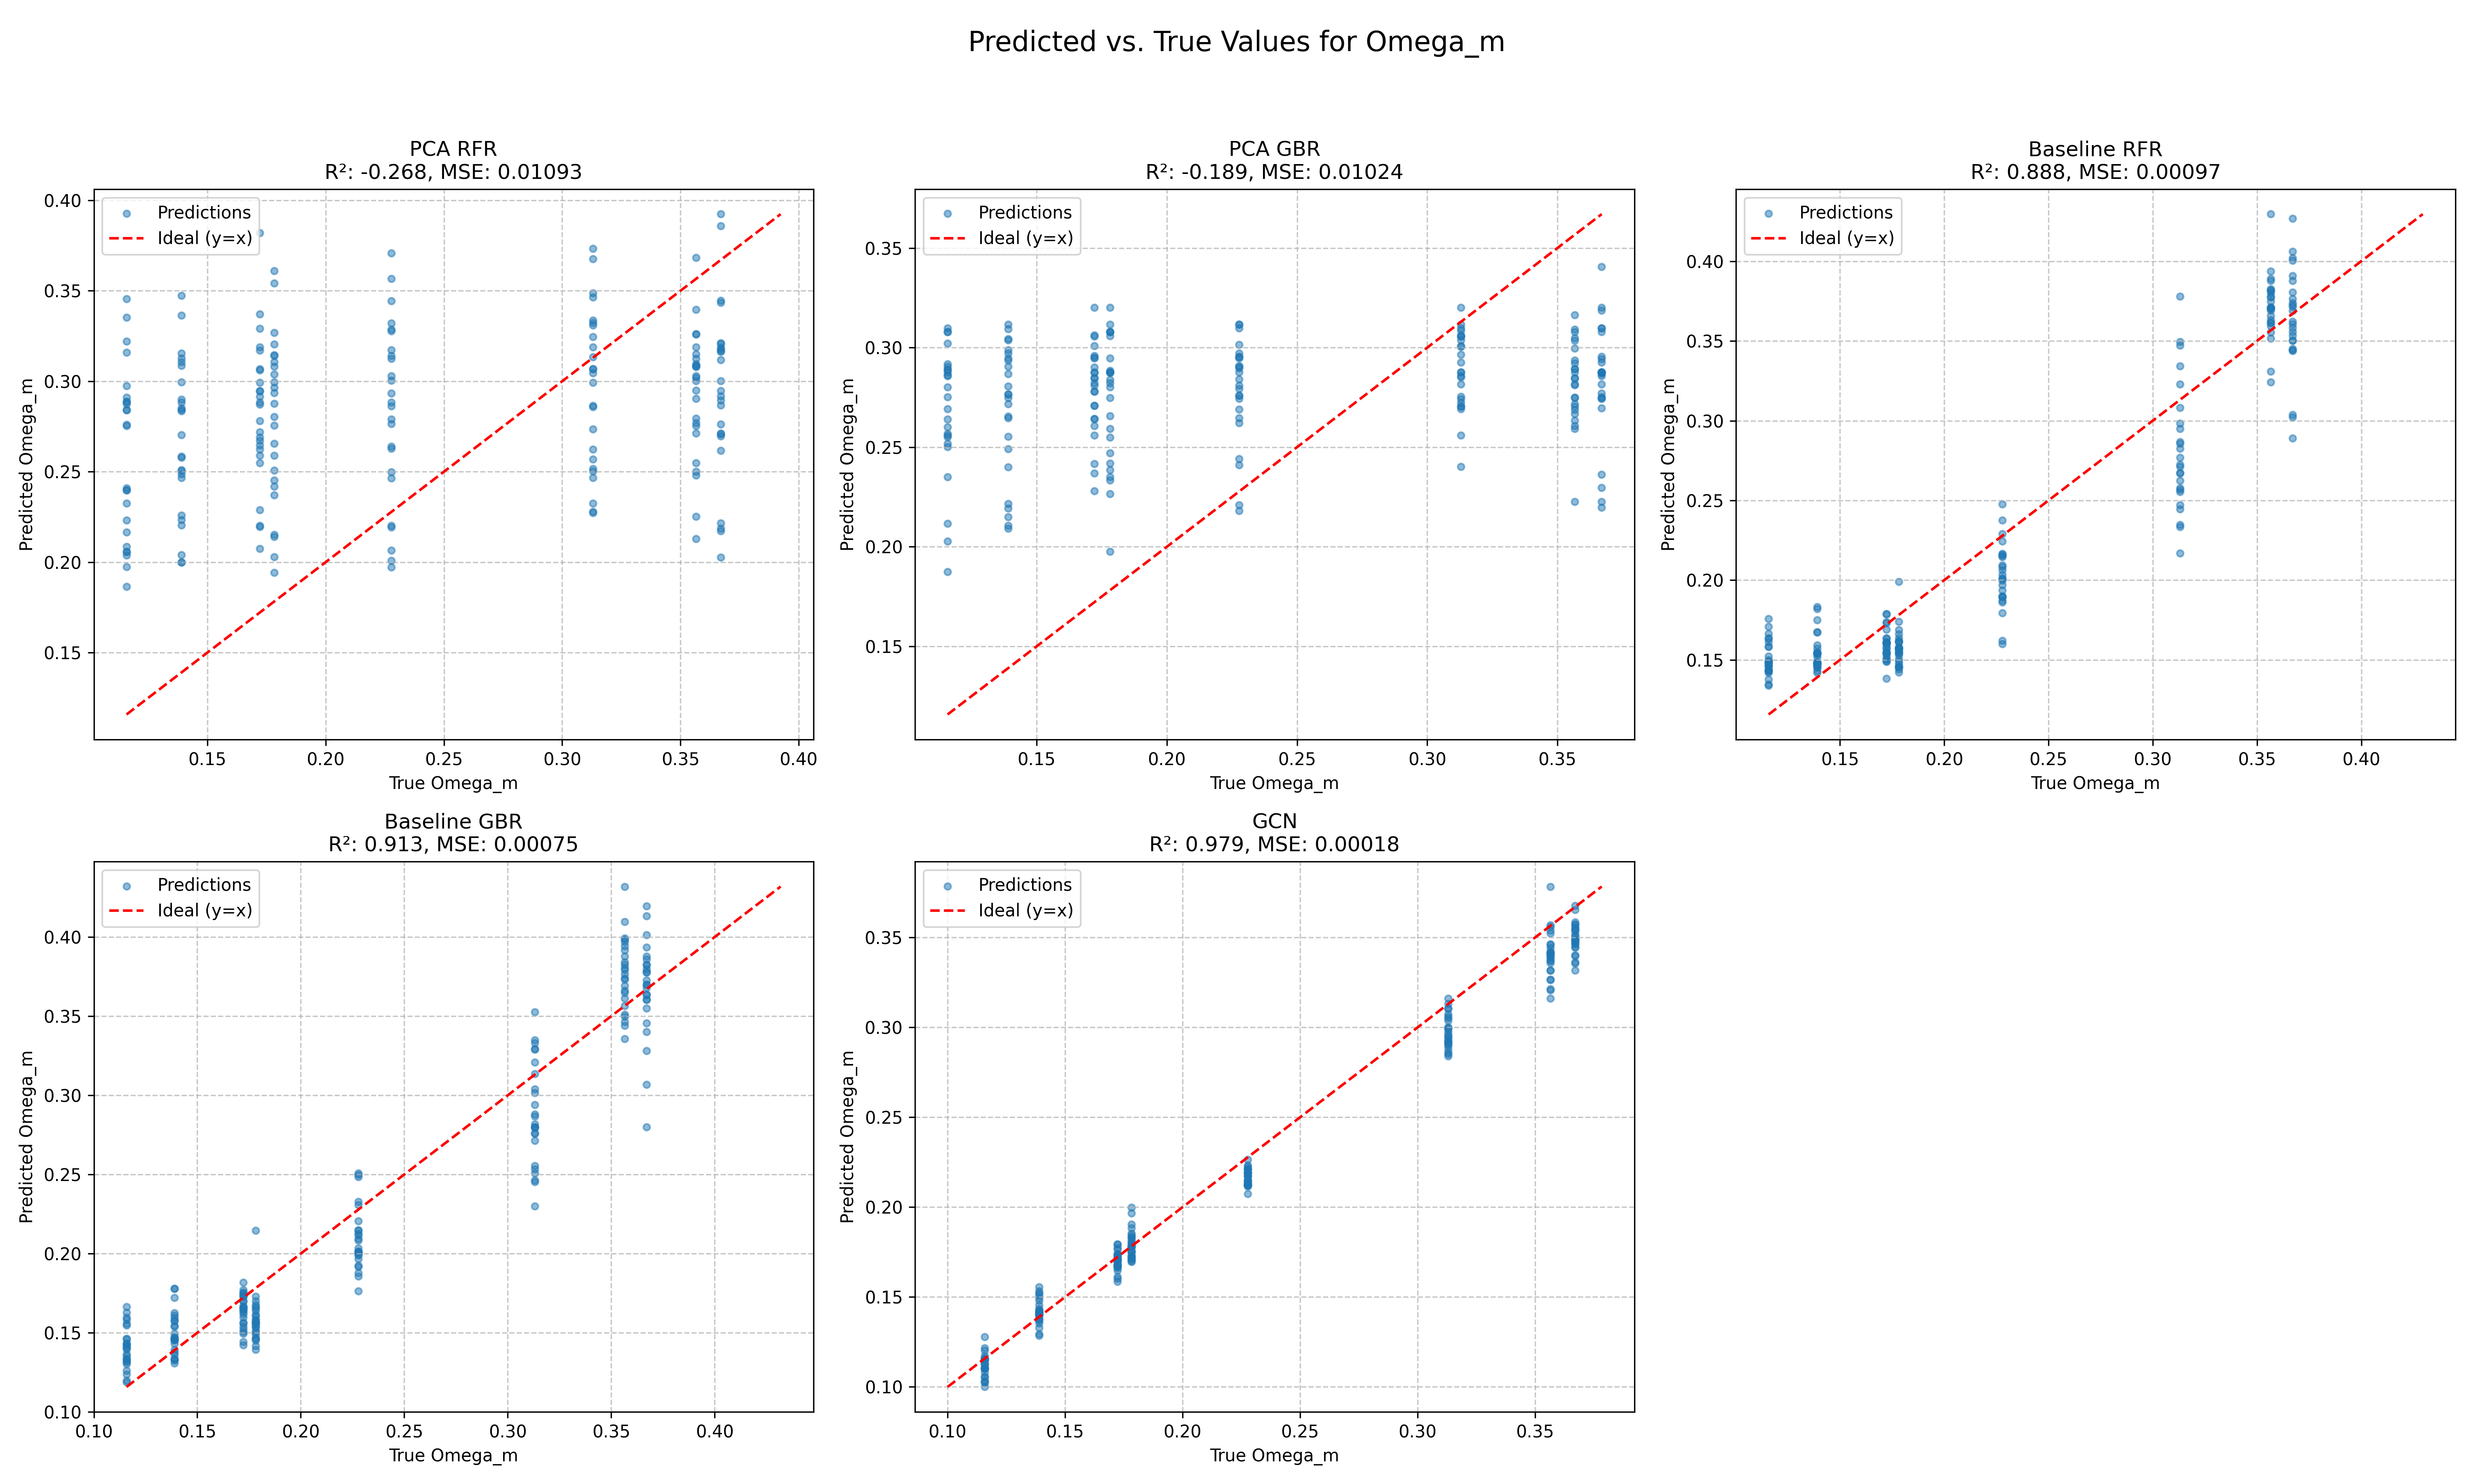
\includegraphics[width=0.5\textwidth]{../input_files/plots/predicted_vs_true_Omega_m_9_20250527-135752.png}
    \caption{Scatter plots of predicted vs. true values of $\Omega_m$ for different models. The GCN and baseline models show a strong positive correlation, while the PCA-engineered feature models show no clear correlation, indicating the superior performance of the former in predicting $\Omega_m$ from merger tree data.}
    \label{fig:predicted_vs_true_omega_m}
\end{figure}

\begin{figure}[h!]
    \centering
    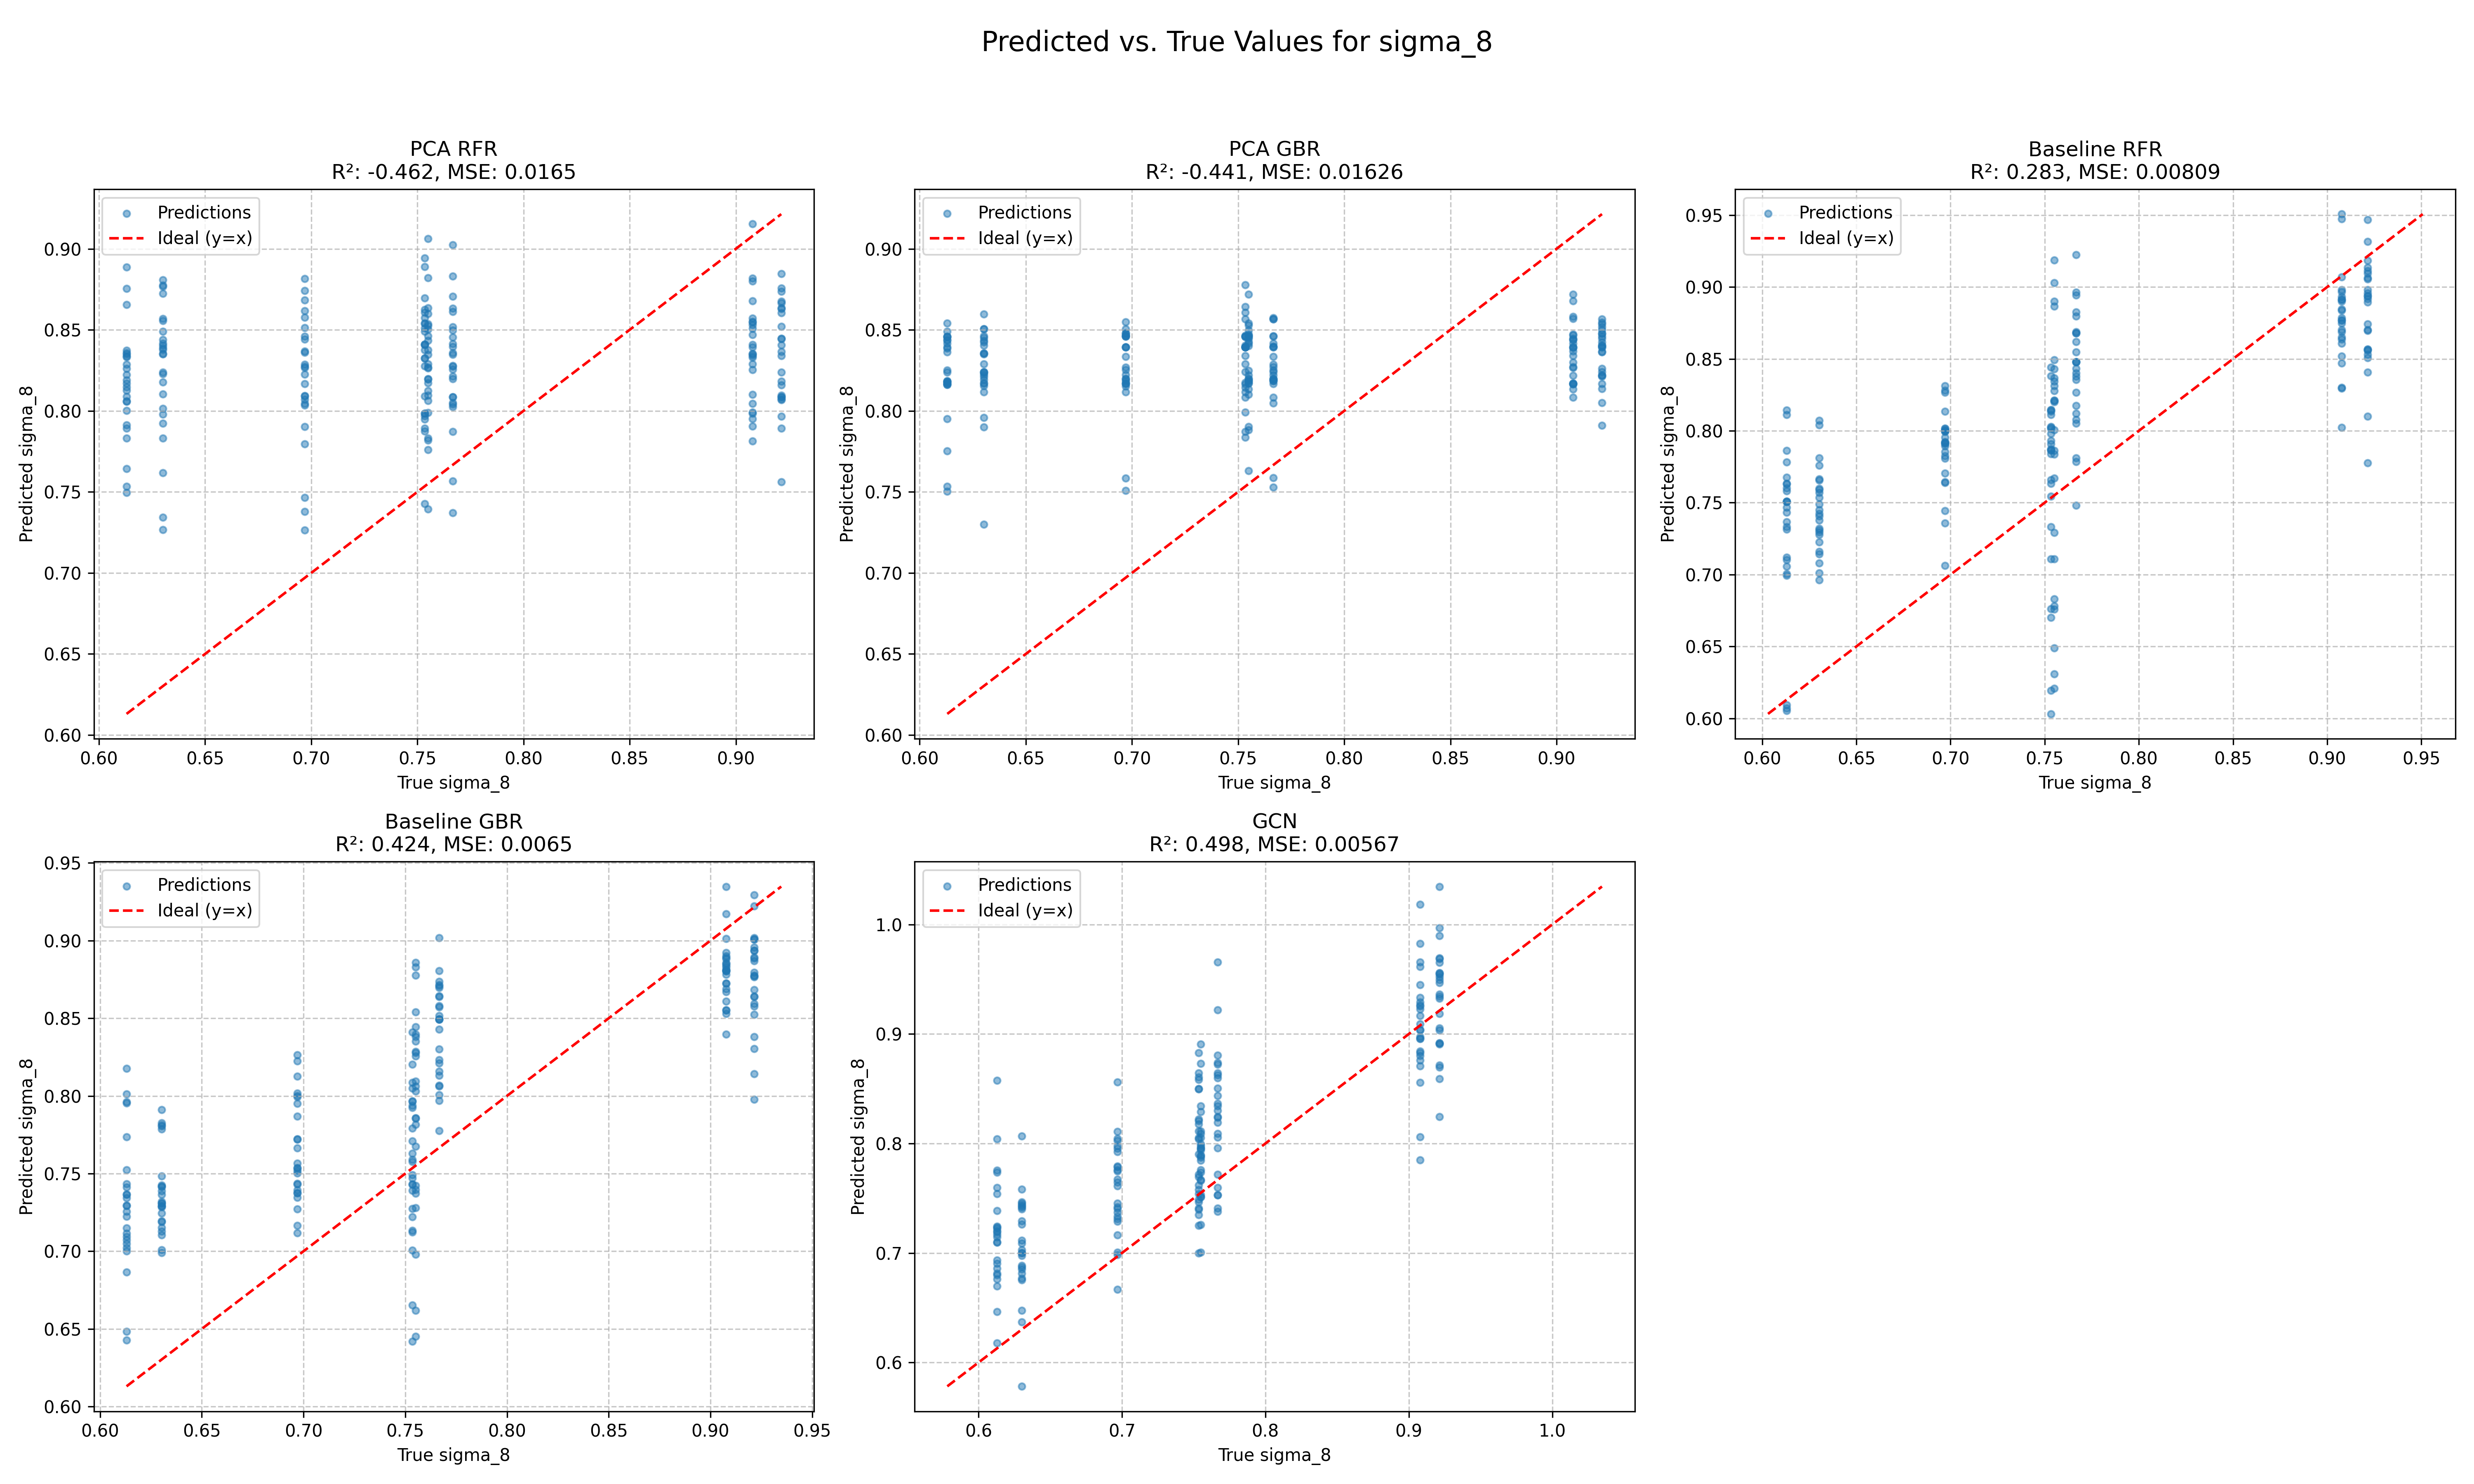
\includegraphics[width=0.5\textwidth]{../input_files/plots/predicted_vs_true_sigma_8_10_20250527-135752.png}
    \caption{Scatter plots of predicted vs. true values for $\sigma_8$ using different feature sets and models: PCA-transformed engineered features with Random Forest Regressor (RFR) and Gradient Boosting Regressor (GBR), baseline aggregated node features with RFR and GBR, and a Graph Convolutional Network (GCN). The GCN and baseline models show positive correlations, whereas the PCA-engineered feature models show little to no correlation, indicating poor predictive performance.}
    \label{fig:predicted_vs_true_sigma_8}
\end{figure}

\subsection{Feature Importance Analysis}

Feature importances were derived for the tree-based models (RFR and GBR). These importances are visualized in Figures \ref{fig:feature_importances_omega_m} and \ref{fig:feature_importances_sigma_8}.

\begin{figure}[h!]
    \centering
    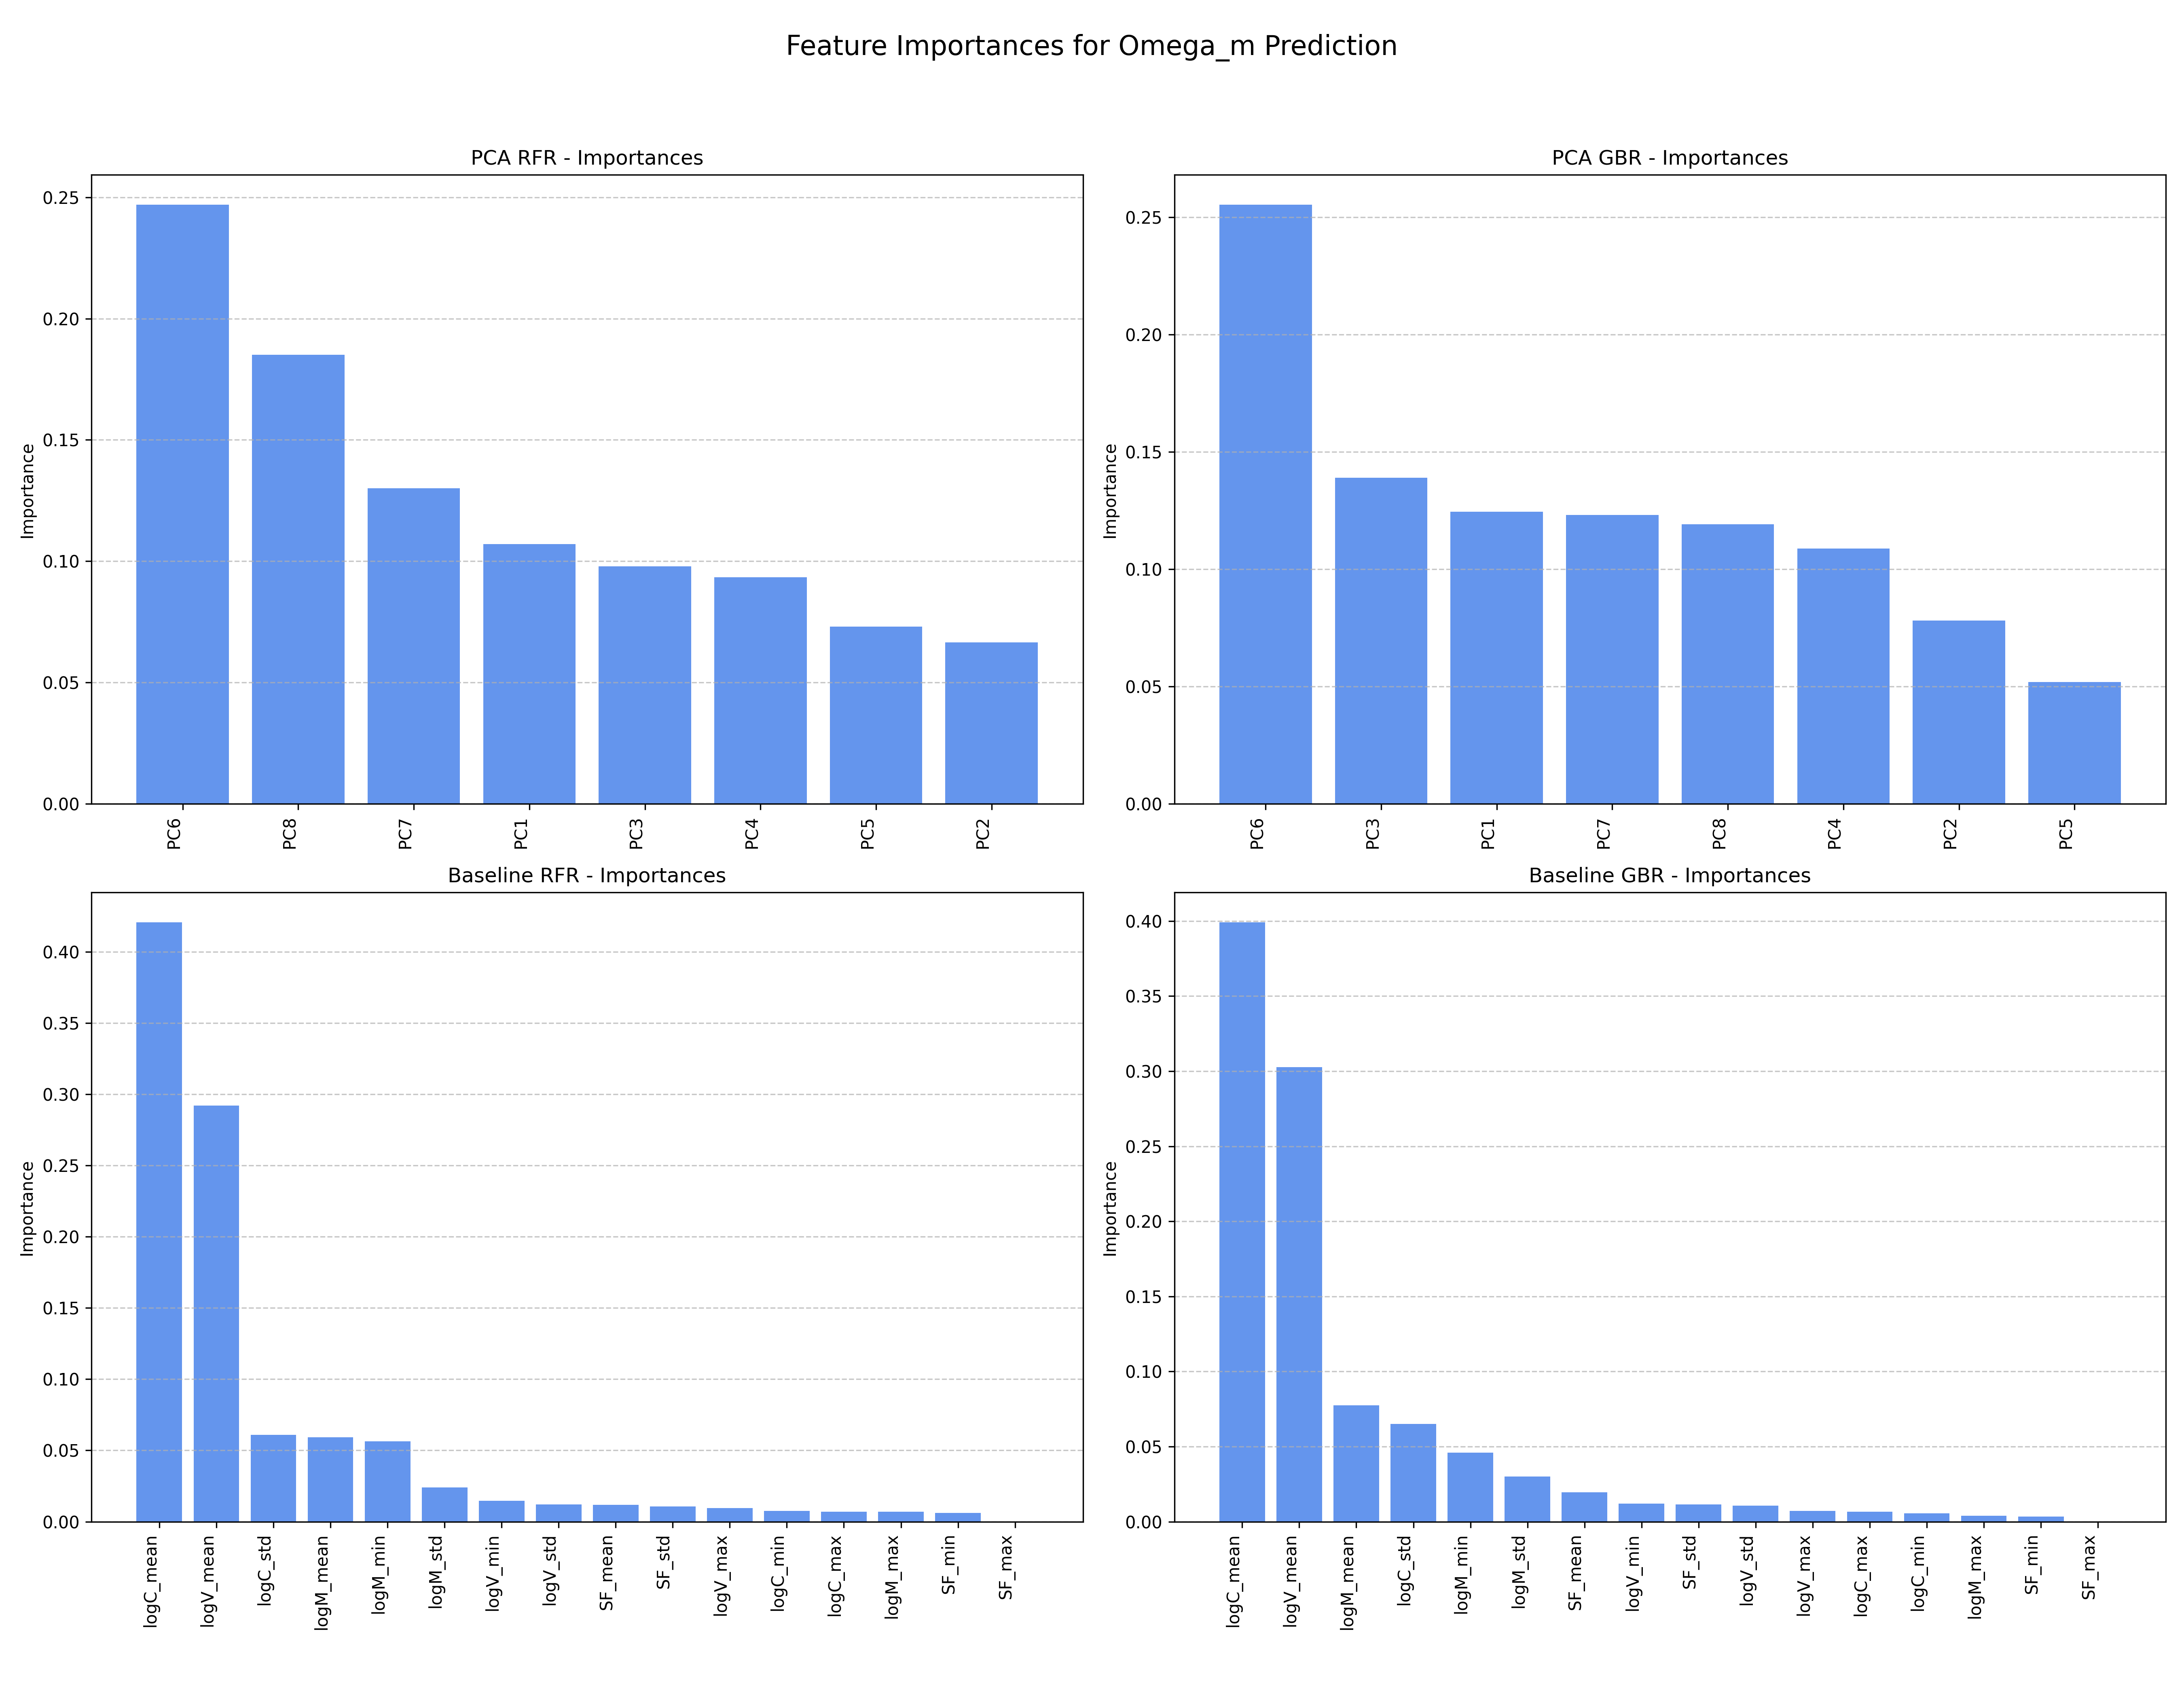
\includegraphics[width=0.5\textwidth]{../input_files/plots/feature_importances_Omega_m_7_20250527-135752.png}
    \caption{Feature importances for predicting $\Omega_m$ using Random Forest Regressor (RFR) and Gradient Boosting Regressor (GBR) models, trained on PCA-transformed engineered features and baseline aggregated node features. The baseline models show that average halo properties such as concentration and Vmax are important predictors, whereas the engineered features show no clear importance.}
    \label{fig:feature_importances_omega_m}
\end{figure}

\begin{figure}[h!]
    \centering
    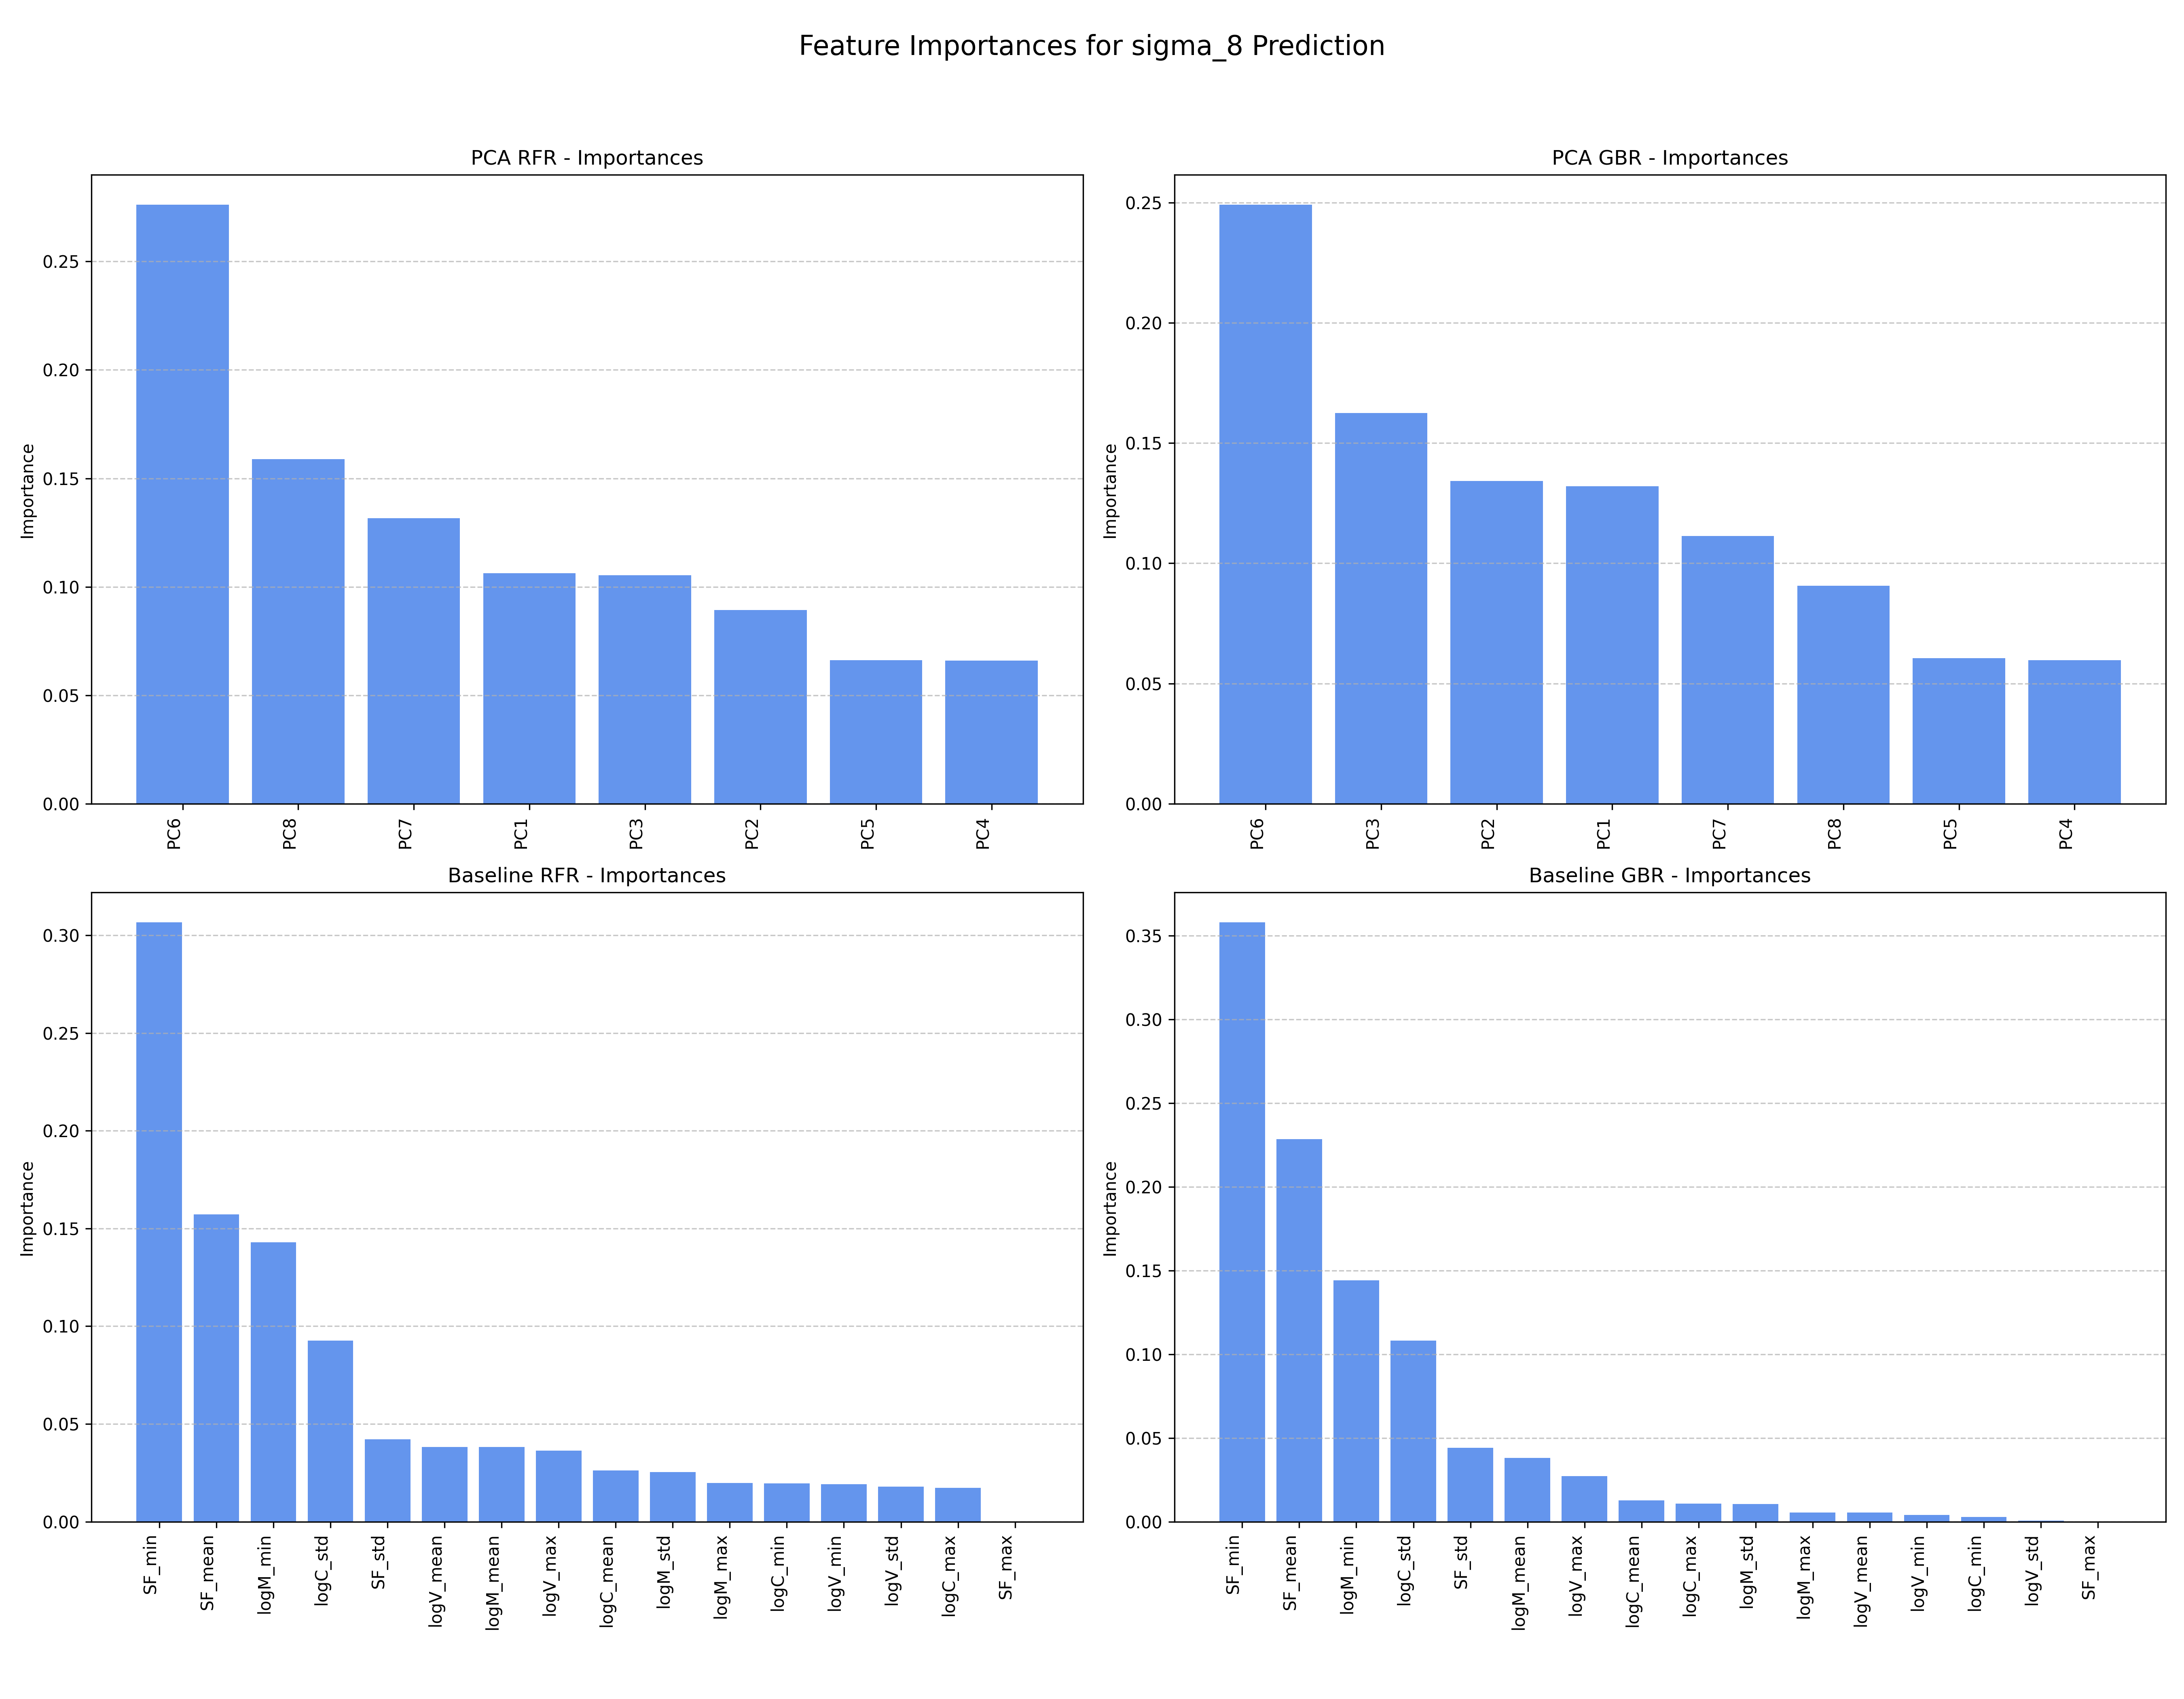
\includegraphics[width=0.5\textwidth]{../input_files/plots/feature_importances_sigma_8_8_20250527-135752.png}
    \caption{Feature importances for predicting $\sigma_8$ using Random Forest Regressor (RFR) and Gradient Boosting Regressor (GBR) models, based on PCA-transformed engineered features and baseline aggregated node features. The baseline models highlight the importance of mean scale factor, mass, and concentration, while PCA-transformed features show varied importances across principal components, but ultimately lead to poor predictive performance.}
    \label{fig:feature_importances_sigma_8}
\end{figure}

\subsubsection{For Baseline Aggregated Node Features}
\begin{itemize}
    \item Predicting $\Omega_m$:
    The RFR model highlighted `SF\_\_mean` (mean scale factor of halos in the tree) as highly important, followed by `logM\_\_mean` (mean log mass) and `logV\_\_mean` (mean log Vmax). The GBR model also emphasized `SF\_\_mean`, `logM\_\_mean`, and `logV\_\_mean`, along with `SF\_\_std` (std of scale factor). This suggests that the average formation time (indicated by scale factor) and average mass/potential well depth of halos in a merger tree are strong indicators of $\Omega_m$.
    \item Predicting $\sigma_8$:
    For RFR, `logM\_\_max` (maximum log mass in the tree), `SF\_\_mean`, and `logC\_\_mean` (mean log concentration) were among the top features. For GBR, `logM\_\_max`, `SF\_\_mean`, and `logM\_\_mean` showed notable importance. The importance of maximum mass and concentration metrics for $\sigma_8$ is plausible, as $\sigma_8$ relates to the amplitude of matter fluctuations, influencing the formation of massive structures and their concentrations.
\end{itemize}

\subsubsection{For Engineered Features + PCA}
The feature importances are for the 8 Principal Components (PC1 to PC8). Predicting $\Omega_m$ and $\sigma_8$: For both targets and both RFR/GBR models, various PCs showed some importance, but no single PC consistently dominated across all models and targets. Interpreting these PC importances directly in terms of the original 24 engineered features is challenging without analyzing the PCA loadings. However, given the overall poor performance of these PCA-reduced features, the specific importances of these PCs are less critical than the observation that they collectively failed to capture predictive signals.

\subsection{Discussion of Engineered Graph Features' Performance}

The most striking outcome of this study is the extremely poor performance of the sophisticated graph spectral and diffusion geometry features, even after PCA. The negative R² values indicate that these features, as implemented and processed, were detrimental to prediction compared to a simple mean prediction. Several factors likely contributed to this:

\subsubsection{Information Loss due to MAX\_NODES\_FOR\_EIGS and Imputation}
A large fraction of graphs (638/800 training, 164/200 testing) had their spectral and diffusion features replaced by NaNs because they exceeded the 500-node limit for eigenvalue computation. These NaNs were then mean-imputed. This imputation strategy, applied to a majority of the data for these 20 features, likely homogenized the feature values, masked true structural variations, and introduced noise, severely degrading their informational content. The distributions plotted in Figures \ref{fig:laplacian_feature_dist}, \ref{fig:diffusion_feature_dist_mean}, \ref{fig:diffusion_feature_dist}, and \ref{fig:diffusion_feature_dist_min} are likely dominated by these imputed means for many graphs.

\subsubsection{Insensitivity of Chosen Features or Aggregation}
The specific spectral moments (mean, std, skewness, kurtosis of eigenvalues, sum of smallest eigenvalues) and the aggregation of diffusion map eigenvectors (mean, max, min pooling) might not be the most sensitive probes of cosmological information encoded in merger tree morphology. These global summaries might average out subtle but crucial structural differences.

\subsubsection{Suboptimal PCA Transformation}
While PCA reduces dimensionality by maximizing variance, it is an unsupervised method. The components that explain most of the variance in the feature space are not necessarily the most predictive for the cosmological parameters. It's possible that information relevant to $\Omega_m$ and $\sigma_8$ was present in lower-variance components that were discarded, or that the linear transformation of PCA was insufficient to disentangle complex relationships.

\subsubsection{Coarseness of Edge Features}
The mean and variance of scale factor differences and log mass ratios might be too simplistic to capture the nuances of merger histories.

\subsubsection{Intrinsic Difficulty}
The relationship between these specific graph-theoretic properties and cosmology might be inherently weak or highly non-linear, making it difficult for traditional regressors to capture, even with perfect features.

The failure of these "classical" geometric deep learning inspired features underscores the challenge in manual feature engineering for complex graph data, especially when computational constraints lead to compromises in feature calculation.

\subsection{Comparison with Baseline Approaches and Physical Implications}

The Baseline Aggregated Node Features significantly outperformed the engineered features. For $\Omega_m$, R² values reached up to 0.9134 (GBR), and for $\sigma_8$, up to 0.4238 (GBR). This implies that simple global statistics of halo properties (average mass, concentration, Vmax, and particularly average scale factor, as indicated by feature importances) within a merger tree are strongly correlated with $\Omega_m$ and moderately correlated with $\sigma_8$. Physically, this suggests that cosmologies with different $\Omega_m$ values produce merger trees with distinguishably different average halo properties and formation epochs. For instance, a higher $\Omega_m$ might lead to earlier formation and thus lower average scale factors in trees, which was picked up by the `SF\_\_mean` feature.

The GCN model demonstrated the best performance overall, achieving an R² of 0.9786 for $\Omega_m$ and 0.4977 for $\sigma_8$. This highlights the strength of GNNs in learning relevant representations directly from raw node features and graph connectivity. GCNs can automatically discover complex, non-linear patterns and feature interactions that are difficult to hand-engineer. The GCN's success, particularly its improvement over the strong baseline, suggests that not only the global average of node properties but also their specific arrangement and relationships within the tree structure (i.e., the graph topology itself) carry cosmological information. The GCN effectively learns a "graph embedding" that is optimized for the prediction task.

The significantly better performance for $\Omega_m$ compared to $\sigma_8$ across all successful methods (Baseline and GCN) suggests that merger tree morphology, as characterized by the input node features, is more sensitive to changes in the matter density parameter than to the amplitude of matter fluctuations on 8 $h^{-1}$Mpc scales.

\subsection{Summary}

In summary, the sophisticated graph spectral and diffusion geometry features performed poorly, likely due to computational limitations and subsequent imputation. Simpler aggregated node features showed significant predictive power, especially for $\Omega_m$, suggesting a strong connection between average halo properties and the matter density parameter. The GCN model achieved the best overall performance, demonstrating the potential of graph neural networks to automatically learn cosmologically relevant information directly from merger tree structures. The GCN's superior performance, particularly for $\Omega_m$, underscores the importance of considering not only global halo properties but also the specific arrangement and relationships within the merger tree structure.

\section{Conclusions}
\label{sec:conclusions}
This study addressed the challenge of extracting cosmological information from dark matter halo merger trees, specifically aiming to predict the matter density parameter ($\Omega_m$) and the amplitude of matter fluctuations ($\sigma_8$). We hypothesized that graph spectral analysis and diffusion geometry could provide meaningful features from merger trees to predict these cosmological parameters. To investigate this, we analyzed a dataset of 1000 merger trees from N-body simulations.

We extracted features using graph spectral analysis, diffusion map embeddings, and astrophysically-motivated edge properties. These engineered features were then used to train regression models, and their performance was compared against a baseline model using aggregated node features and a Graph Convolutional Network (GCN). A key challenge was the computational cost of eigenvalue decomposition for large graphs, leading to a significant number of missing values that were subsequently imputed.

Our results indicated that the engineered graph spectral and diffusion geometry features performed poorly, likely due to the computational limitations during feature extraction and the subsequent imputation of missing values. Simpler aggregated node features, representing global statistics of halo properties, showed significant predictive power, especially for $\Omega_m$. The GCN model achieved the best overall performance, demonstrating the potential of graph neural networks to automatically learn cosmologically relevant information directly from merger tree structures. The GCN showed a strong predictive capability for $\Omega_m$, while the baseline models also showed a strong correlation with this parameter. For $\sigma_8$, the GCN model again showed the best performance, but with a lower R² than for $\Omega_m$. The baseline models also exhibited a positive but weaker correlation, while the PCA-engineered feature models again showed no discernible correlation.

From these results, we learned that sophisticated graph signal processing techniques, when limited by computational constraints and imputation, may not outperform simpler feature engineering approaches. The success of the aggregated node features suggests that the average halo properties within a merger tree are strongly correlated with $\Omega_m$. Furthermore, the superior performance of the GCN highlights the potential of geometric deep learning to automatically learn cosmologically relevant information from merger tree structures, capturing complex relationships that are difficult to hand-engineer. The study also indicates that merger tree morphology, as characterized by the input node features, is more sensitive to changes in the matter density parameter than to the amplitude of matter fluctuations. This underscores the challenges of manual feature engineering in complex graph data and the promise of geometric deep learning for cosmological inference.

\bibliography{bibliography}{}
\bibliographystyle{aasjournal}

\end{document}
